%definira klasu dokumenta 
\documentclass[12pt]{report} 

%prostor izmedu naredbi \documentclass i \begin{document} se zove uvod. U njemu se nalaze naredbe koje se odnose na cijeli dokument

%osnovni LaTex ne može riješiti sve probleme, pa se koriste različiti paketi koji olakšavaju izradu željenog dokumenta
\usepackage[croatian]{babel} 
\usepackage{amssymb}
\usepackage{amsmath}
\usepackage{txfonts}
\usepackage{mathdots}
\usepackage{titlesec}
\usepackage{array}
\usepackage{lastpage}
\usepackage{etoolbox}
\usepackage{tabularray}
\usepackage{color, colortbl}
\usepackage{adjustbox}
\usepackage{geometry}
\usepackage[classicReIm]{kpfonts}
\usepackage{hyperref}
\usepackage{fancyhdr}

\usepackage{float}
\usepackage{setspace}
\restylefloat{table}


\patchcmd{\chapter}{\thispagestyle{plain}}{\thispagestyle{fancy}}{}{} %redefiniranje stila stranice u paketu fancyhdr

%oblik naslova poglavlja
\titleformat{\chapter}{\normalfont\huge\bfseries}{\thechapter.}{20pt}{\Huge}
\titlespacing{\chapter}{0pt}{0pt}{40pt}


\linespread{1.3} %razmak između redaka

\geometry{a4paper, left=1in, top=1in,}  %oblik stranice

\hypersetup{ colorlinks, citecolor=black, filecolor=black, linkcolor=black,	urlcolor=black }   %izgled poveznice


%prored smanjen između redaka u nabrajanjima i popisima
\newenvironment{packed_enum}{
	\begin{enumerate}
		\setlength{\itemsep}{0pt}
		\setlength{\parskip}{0pt}
		\setlength{\parsep}{0pt}
	}{\end{enumerate}}

\newenvironment{packed_item}{
	\begin{itemize}
		\setlength{\itemsep}{0pt}
		\setlength{\parskip}{0pt}
		\setlength{\parsep}{0pt}
	}{\end{itemize}}




%boja za privatni i udaljeni kljuc u tablicama
\definecolor{LightBlue}{rgb}{0.9,0.9,1}
\definecolor{LightGreen}{rgb}{0.9,1,0.9}

%Promjena teksta za dugačke tablice
\DefTblrTemplate{contfoot-text}{normal}{Nastavljeno na idućoj stranici}
\SetTblrTemplate{contfoot-text}{normal}
\DefTblrTemplate{conthead-text}{normal}{(Nastavljeno)}
\SetTblrTemplate{conthead-text}{normal}
\DefTblrTemplate{middlehead,lasthead}{normal}{Nastavljeno od prethodne stranice}
\SetTblrTemplate{middlehead,lasthead}{normal}

%podesavanje zaglavlja i podnožja

\pagestyle{fancy}
\lhead{Programsko inženjerstvo}
\rhead{$<$Projektni zadatak$>$}
\lfoot{$<$Naziv grupe$>$}
\cfoot{stranica \thepage/\pageref{LastPage}}
\rfoot{\today}
\renewcommand{\headrulewidth}{0.2pt}
\renewcommand{\footrulewidth}{0.2pt}


\begin{document} 
	
	
	
	\begin{titlepage}
		\begin{center}
			\vspace*{\stretch{1.0}} %u kombinaciji s ostalim \vspace naredbama definira razmak između redaka teksta
			\LARGE Programsko inženjerstvo\\
			\large Ak. god. 2020./2021.\\
			
			\vspace*{\stretch{3.0}}
			
			\huge $<$Naziv projekta$>$\\
			\Large Dokumentacija, Rev. \textit{$<$1 ili 2$>$}\\
			
			\vspace*{\stretch{12.0}}
			\normalsize
			Grupa: \textit{$<$Naziv grupe$>$}\\
			Voditelj: \textit{$<$Ime i prezime voditelja$>$}\\
			
			
			\vspace*{\stretch{1.0}}
			Datum predaje: \textit{$<$dan$>$. $<$mjesec$>$. $<$godina$>$.}\\
	
			\vspace*{\stretch{4.0}}
			
			Nastavnik: \textit{$<$Ime i prezime nastavnika zaduženog za vašu grupu$>$}\\
		
		\end{center}

	
	\end{titlepage}

	
	\tableofcontents


	\chapter{Dnevnik promjena dokumentacije}
		
		\textbf{\textit{Kontinuirano osvježavanje}}\\
				
		
		\begin{longtblr}[
				label=none
			]{
				width = \textwidth, 
				colspec={|X[2]|X[13]|X[3]|X[3]|}, 
				rowhead = 1
			}
			\hline
			\textbf{Rev.}	& \textbf{Opis promjene/dodatka} & \textbf{Autori} & \textbf{Datum}\\[3pt] \hline
			0.1 & Napravljen predložak.	& * & 22.08.2013. 		\\[3pt] \hline 
			0.2	& Dopisane upute za povijest dokumentacije.\newline Dodane reference. & * & 24.08.2013. 	\\[3pt] \hline 
			0.5 & Dodan \textit{Use Case} dijagram i jedan sekvencijski dijagram, funkcionalni i nefunkcionalni zahtjevi i dodatak A & * & 25.08.2013. \\[3pt] \hline 
			0.6 & Arhitektura i dizajn sustava, algoritmi i strukture podataka & * & 26.08.2013. \\[3pt] \hline 
			0.8 & Povijest rada i trenutni status implementacije,\newline Zaključci i plan daljnjeg rada & * & 28.08.2013. \\[3pt] \hline 
			0.9 & Opisi obrazaca uporabe & * & 07.09.2013. \\[3pt] \hline 
			0.10 & Preveden uvod & * & 08.09.2013. \\[3pt] \hline 
			0.11 & Sekvencijski dijagrami & * & 09.09.2013. \\[3pt] \hline 
			0.12.1 & Započeo dijagrame razreda & * & 10.09.2013. \\[3pt] \hline 
			0.12.2 & Nastavak dijagrama razreda & * & 11.09.2013. \\[3pt] \hline 
			\textbf{1.0} & Verzija samo s bitnim dijelovima za 1. ciklus & * & 11.09.2013. \\[3pt] \hline 
			1.1 & Uređivanje teksta -- funkcionalni i nefunkcionalni zahtjevi & * \newline * & 14.09.2013. \\[3pt] \hline 
			1.2 & Manje izmjene:Timer - Brojilo vremena & * & 15.09.2013. \\[3pt] \hline 
			1.3 & Popravljeni dijagrami obrazaca uporabe & * & 15.09.2013. \\[3pt] \hline 
			1.5 & Generalna revizija strukture dokumenta & * & 19.09.2013. \\[3pt] \hline 
			1.5.1 & Manja revizija (dijagram razmještaja) & * & 20.09.2013. \\[3pt] \hline 
			\textbf{2.0} & Konačni tekst predloška dokumentacije  & * & 28.09.2013. \\[3pt] \hline 
			&  &  & \\[3pt] \hline	
		\end{longtblr}
	
	
		\textit{Moraju postojati glavne revizije dokumenata 1.0 i 2.0 na kraju prvog i drugog ciklusa. Između tih revizija mogu postojati manje revizije već prema tome kako se dokument bude nadopunjavao. Očekuje se da nakon svake značajnije promjene (dodatka, izmjene, uklanjanja dijelova teksta i popratnih grafičkih sadržaja) dokumenta se to zabilježi kao revizija. Npr., revizije unutar prvog ciklusa će imati oznake 0.1, 0.2, …, 0.9, 0.10, 0.11.. sve do konačne revizije prvog ciklusa 1.0. U drugom ciklusu se nastavlja s revizijama 1.1, 1.2, itd.}
	\chapter{Opis projektnog zadatka}
		
		%\textbf{\textit{dio 1. revizije}}\\
		
		\textit{Na osnovi projektnog zadatka detaljno opisati korisničke zahtjeve. Što jasnije opisati cilj projektnog zadatka, razraditi problematiku zadatka, dodati nove aspekte problema i potencijalnih rješenja. Očekuje se minimalno 3, a poželjno 4-5 stranica opisa.	Teme koje treba dodatno razraditi u ovom poglavlju su:}
		\begin{packed_item}
			\item \textit{potencijalna korist ovog projekta}
			\item \textit{postojeća slična rješenja (istražiti i ukratko opisati razlike u odnosu na zadani zadatak). Dodajte slike koja predočavaju slična rješenja.}
			\item \textit{skup korisnika koji bi mogao biti zainteresiran za ostvareno rješenje.}
			\item \textit{mogućnost prilagodbe rješenja }
			\item \textit{opseg projektnog zadatka}
			\item \textit{moguće nadogradnje projektnog zadatka}
		\end{packed_item}
		
		\textit{Za pomoć pogledati reference navedene u poglavlju „Popis literature“, a po potrebi konzultirati sadržaj na internetu koji nudi dobre smjernice u tom pogledu.}
		\eject
		
	\chapter{Specifikacija programske potpore}
		
	\section{Funkcionalni zahtjevi}

			%\textbf{\textit{dio 1. revizije}}\\
					
			\noindent \textbf{Dionici:}
			
			\begin{packed_enum}
				
				\item Dionik 1
				\item Dionik 2				
				\item ...
				
			\end{packed_enum}
			
			\noindent \textbf{Aktori i njihovi funkcionalni zahtjevi:}
			
			
			\begin{packed_enum}
				\item  \underbar{Aktor 1 (inicijator) može:}
				
				\begin{packed_enum}
					
					\item funkcionalnost 1
					\item funkcionalnost 2
					\begin{packed_enum}
						
						\item  podfunkcionalnost 1 
						\item  podfunkcionalnost 2
				
					\end{packed_enum}
					\item  funkcionalnost 3
					
				\end{packed_enum}
			
				\item  \underbar{Aktor 2 (sudionik) može:}
				
				\begin{packed_enum}
					
					\item funkcionalnost 1
					\item funkcionalnost 2
					
				\end{packed_enum}
			\end{packed_enum}
			
			\eject 
			
			
				
			\subsection{Obrasci uporabe}
				
				%\textbf{\textit{dio 1. revizije}}
				
				\subsubsection{Opis obrazaca uporabe}			

					\noindent \underbar{\textbf{UC$<$broj obrasca$>$ -$<$ime obrasca$>$}}
					\begin{packed_item}
	
						\item \textbf{Glavni sudionik: }$<$sudionik$>$
						\item  \textbf{Cilj:} $<$cilj$>$
						\item  \textbf{Sudionici:} $<$sudionici$>$
						\item  \textbf{Preduvjet:} $<$preduvjet$>$
						\item  \textbf{Opis osnovnog tijeka:}
						
						\item[] \begin{packed_enum}
	
							\item $<$opis korak jedan$>$
							\item $<$opis korak dva$>$
							\item $<$opis korak tri$>$
							\item $<$opis korak četiri$>$
							\item $<$opis korak pet$>$
						\end{packed_enum}
						
						\item  \textbf{Opis mogućih odstupanja:}
						
						\item[] \begin{packed_item}
	
							\item[2.a] $<$opis mogućeg scenarija odstupanja u koraku 2$>$
							\item[] \begin{packed_enum}
								
								\item $<$opis rješenja mogućeg scenarija korak 1$>$
								\item $<$opis rješenja mogućeg scenarija korak 2$>$
								
							\end{packed_enum}
							\item[2.b] $<$opis mogućeg scenarija odstupanja u koraku 2$>$
							\item[3.a] $<$opis mogućeg scenarija odstupanja  u koraku 3$>$
							
						\end{packed_item}
					\end{packed_item}
				
					
				\subsubsection{Dijagrami obrazaca uporabe}
					
					\textit{Prikazati odnos aktora i obrazaca uporabe odgovarajućim UML dijagramom. Nije nužno nacrtati sve na jednom dijagramu. Modelirati po razinama apstrakcije i skupovima srodnih funkcionalnosti.}
				\eject
				
			\subsection{Sekvencijski dijagrami}
				
				%\textbf{\textit{dio 1. revizije}}\\
				
				\textit{Nacrtati sekvencijske dijagrame koji modeliraju najvažnije dijelove sustava (max. 4 dijagrama). Ukoliko postoji nedoumica oko odabira, razjasniti s asistentom. Uz svaki dijagram napisati detaljni opis dijagrama.}
				\eject
	
		\section{Ostali zahtjevi}
		
			%\textbf{\textit{dio 1. revizije}}\\
		 
	\chapter{Arhitektura i dizajn sustava}
		
		%\textbf{\textit{dio 1. revizije}}\\

		%\textit{ Potrebno je opisati stil arhitekture te identificirati: podsustave, preslikavanje na radnu platformu, spremišta podataka, mrežne protokole, globalni upravljački tok i sklopovsko-programske zahtjeve. Po točkama razraditi i popratiti odgovarajućim skicama:}
	%\begin{itemize}
		%\item 	\textit{izbor arhitekture temeljem principa oblikovanja pokazanih na predavanjima (objasniti zašto ste baš odabrali takvu arhitekturu)}
		%\item 	\textit{organizaciju sustava s najviše razine apstrakcije (npr. klijent-poslužitelj, baza podataka, datotečni sustav, grafičko sučelje)}
		%\item 	\textit{organizaciju aplikacije (npr. slojevi frontend i backend, MVC arhitektura) }		
	%\end{itemize}
				
		Arhitektura naše aplikacije zajedno s vanjskim resursima (bazom) na najvišoj razni apstrakcije odgovara troslojnoj klijent-poslužitelj arhitekturi sa sljedećim slojevima:
		\begin{itemize}
			\item Prezentacijski sloj (Frontend)
			\item Sloj poslovne logike (Backend)
			\item Podatkovni sloj (Baza podataka)
		\end{itemize}

		\begin{figure}[H]
			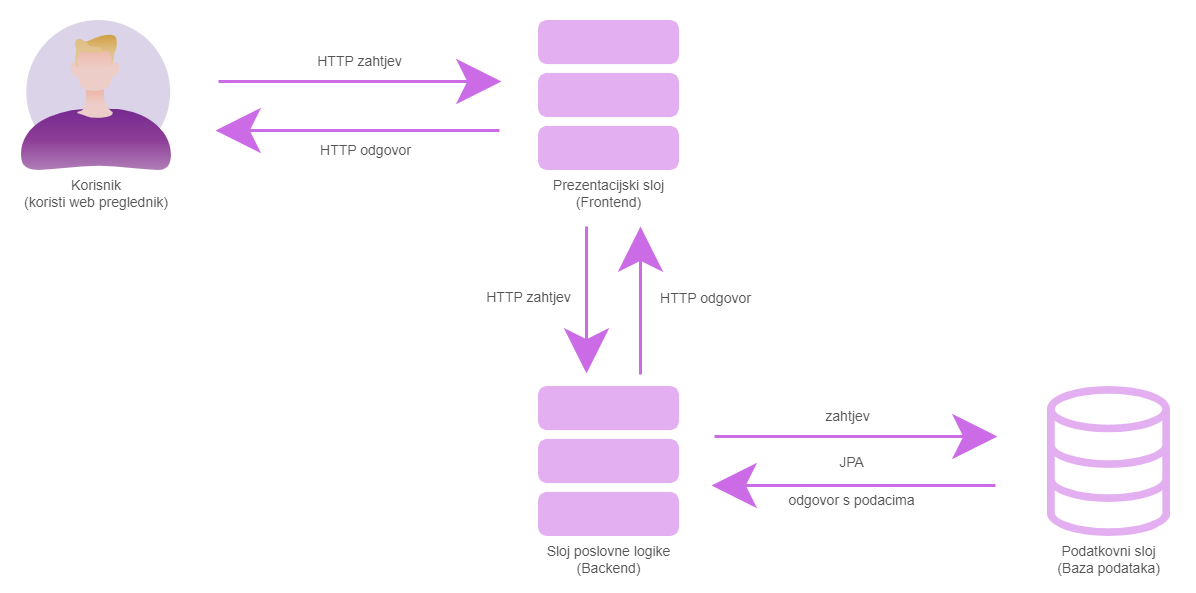
\includegraphics[width=\textwidth,height=0.4\textheight]{slike/Arhitektura.png}
			\centering
			\caption{Arhitektura sustava}
			\label{fig:Arhitektura}
		\end{figure}

		\eject

		Općenito govoreći, prezentacijski sloj tj. frontend zadužen je za prikaz stranice korisniku i omogućavanje rada s istom. S druge strane, sloj poslovne logike tj. backend zadužena je za razne izračune i interakciju s bazom. U ovom pogledu, sloj poslovne logike služi kao spona između prezentacijskog sloja i podatkovnog sloja koja pritom obavlja sve akcije neprikladne za izvođenje na klijentovom računalu.\\[2pt]

		Kada korisnik u web preglednik unese URL naše stranice, web preglednik pristupa našoj aplikaciji slanjem HTTP GET zahtjeva prezentacijskom sloju. Prezentacijski sloj u odgovoru šalje sve potrebne podatke za prikaz korisničkog sučelja - naše stranice.
		Kada korisniku treba poslužiti neki sadržaj koji nije pohranjen na prezentacijskom sloju (npr. aktivne donacije, podatci o korisniku i oglasima), prezentacijski sloj sloju poslovne logike šalje HTTP zahtjev - npr. GET zahtjev s ciljem dohvata podataka o djeci korisnika.
		Komunikacija između prezentacijskog sloja i sloja poslovne logike odvija se po REST načelima.\\[2pt]

		Sloj poslovne logike potreban je za kompliciranije izračune, dohvat i izmjenu podataka te odgovaranje na zahtjeve pristigle od strane prezentacijskog sloja.
		Podatkovni sloj tj. baza podataka služi za pohranu svih potrebnih podataka (npr. podataka o registriranim korisnicima, oglasima i predmetima). Pri radu naše aplikacije, s bazom podataka komunicira isključivo sloj poslovne logike tj. backend - ako prezentacijskom sloju trebaju određeni podaci, poslat će zahtjev sloju poslovne logike te u idealnom slučaju u odgovoru dobiti tražene podatke. Pritom, JPA služi za objektno/relacijsko mapiranje (ORM) zahtjeva backenda u SQL upite pomoću kojih je moguće komunicirati s bazom.\\[2pt]

		Dodatno, i prezentacijski sloj i sloj poslovne logike interno imaju vlastitu podjelu - sloj poslovne logike možemo podijeliti na 3 glavne komponente: kontroleri, servisi i repozitoriji (sloj pristupa podacima). Sličnu podjelu moguće je uočiti i na prezentacijskom sloju. Baza podataka vanjski je resurs koji naša aplikacija koristi.

		\eject

		Prezentacijski sloj tj. frontend izrađen je koristeći programski jezik Javascript zajedno s "markup" jezikom HTML, CSS-om i radnim okvirom React. Zbog korištenja radnog okvira React koji omogućava provođenje brojnih izračuna i funkcionalnosti na klijentovom računalu, možemo reći da je u pitanju "debeli" klijent.
		Sloj poslovne logike tj. backend izrađen je koristeći programski jezik Java zajedno s radnim okvirom Java Spring Boot. Za prevođenje zahtjeva backenda u ispravne SQL upite korišten je JPA - Java Persistence API.
		Shema baze podataka izrađena je koristeći alat ERDplus, a sama baza podataka izrađena je koristeći sustav za upravljanje bazama PostgreSQL.

		\eject
		\section{Baza podataka}
			
		Za naš zadatak odabrali smo koristiti relacijsku bazu podataka kako bismo što učinkovitije i realističnije prikazali potreban sustav, 
		ali isto tako i zato što s relacijskim bazama podataka imamo najviše iskustva, primarno stečenog na kolegiju Baze podataka.
		Baza podataka sastoji se od nekolicine relacija tj. tablica definiranih imenom relacije i skupom atributa relacije.
		Među atributima relacije obvezno se nalazi primarni ključ, a ponekad i strani ključevi koji povezuju tu relaciju s ostalima.
		Bazu koristimo za pohranu, izmjenu i dohvat potrebnih podataka.

		\vspace{15pt}

		Baza podataka naše aplikacije sastoji se od sljedećih relacija:
		\begin{packed_item}
			\item User
			\item Child
			\item Category
			\item Subcategory
			\item isInCategory
			\item isInSubcategory
			\item Item
			\item Donation
			\item donatedToUser
		\end{packed_item}
			
		%\textit{Potrebno je opisati koju vrstu i implementaciju baze podataka ste odabrali, glavne komponente od kojih se sastoji i slično.}
			\eject
			\subsection{Opis tablica}
			
				\textit{Primarni ključevi relacija označeni su zelenom bojom, a strani ključevi plavom bojom. }
				%\textit{Svaku tablicu je potrebno opisati po zadanom predlošku. Lijevo se nalazi točno ime varijable u bazi podataka, u sredini se nalazi tip podataka, a desno se nalazi opis varijable. Svjetlozelenom bojom označite primarni ključ. Svjetlo plavom označite strani ključ}
				\newline
				\newline
				Relacija \textbf{User} služi za pohranu podataka o registriranome korisniku aplikacije. Sadrži atribute: email, userName, userSurname, password, userLocation, isAccountVerified i canDonate. Relacija je povezana s relacijom Child, relacijom Donation i relacijom donatedToUser.
				\begin{longtblr}[
					label=none,
					entry=none
					]{
						width = \textwidth,
						colspec={|X[10,l]|X[6, l]|X[20, l]|}, 
						rowhead = 1,
					}
					\hline \multicolumn{3}{|c|}{\textbf{User}}	 \\ \hline[3pt]
					\SetCell{LightGreen}email & VARCHAR	& Email adresa korisnika  	\\ \hline
					userName	& VARCHAR & Ime korisnika	\\ \hline 
					userSurname & VARCHAR & Prezime korisnika  \\ \hline 
					password & VARCHAR	& Lozinka korisnika 		\\ \hline 
					userLocation & VARCHAR & Lokacija korisnika 	\\ \hline
					isAccountVerified & BOOLEAN & Oznaka je li korisnik verificiran \\ \hline
					canDonate & BOOLEAN & Oznaka može li korisnik donirati \\ \hline
				\end{longtblr}
				\eject
				Relacija \textbf{Child} služi za pohranu podataka o djetetu registriranog korisnika aplikacije. Sadrži atribute: email, childId, childName, childSex, childAge i predictedBirthDate. Relacija je povezana s relacijom User, relacijom isInCategory i relacijom isInSubcategory.
				\begin{longtblr}[
					label=none,
					entry=none
					]{
						width = \textwidth,
						colspec={|X[10,l]|X[6, l]|X[20, l]|}, 
						rowhead = 1,
					}
					\hline \multicolumn{3}{|c|}{\textbf{Child}}	 \\ \hline[3pt]
					\SetCell{LightGreen}childId & INT	& Generirani id djeteta  	\\ \hline
					\SetCell{LightGreen} email	& VARCHAR & Email adresa roditelja - također strani ključ	\\ \hline 
					childName & VARCHAR & Ime djeteta  \\ \hline 
					childSex & VARCHAR	& Spol djeteta		\\ \hline 
					childAge & INT & Dob djeteta	\\ \hline
					predictedBirthDate & DATE & Predviđeni datum rođenja djeteta \\ \hline
				\end{longtblr}

				Relacija \textbf{Category} služi za pohranu podataka o određenoj kategoriji. Sadrži atribut: categoryName. Relacija je povezana s relacijom isInCategory, relacijom Subcategory i relacijom Item.
				\begin{longtblr}[
					label=none,
					entry=none
					]{
						width = \textwidth,
						colspec={|X[10,l]|X[6, l]|X[20, l]|}, 
						rowhead = 1,
					}
					\hline \multicolumn{3}{|c|}{\textbf{Category}}	 \\ \hline[3pt]
					\SetCell{LightGreen} categoryName & VARCHAR	& Ime kategorije  	\\ \hline
				\end{longtblr}

				Relacija \textbf{Subcategory} služi za pohranu podataka o određenoj potkategoriji. Sadrži atribute: subcategoryName, itemDuration i categoryName. Relacija je povezana s relacijom isInSubcategory, relacijom Category i relacijom Item.
				\begin{longtblr}[
					label=none,
					entry=none
					]{
						width = \textwidth,
						colspec={|X[10,l]|X[6, l]|X[20, l]|}, 
						rowhead = 1,
					}
					\hline \multicolumn{3}{|c|}{\textbf{Subcategory}}	 \\ \hline[3pt]
					\SetCell{LightGreen} subcategoryName & VARCHAR	& Ime potkategorije 	\\ \hline
					itemDuration & INT & Predviđeni rok uporabe predmeta iz potkategorije u godinama \\ \hline
					\SetCell{LightBlue} categoryName & VARCHAR & Ime roditeljske kategorije \\ \hline
				\end{longtblr}

				Relacija \textbf{isInCategory} nastala je iz veze N:N između relacija Child i Category i služi za povezivanje istih. Sadrži atribute: childId, email i categoryName. Relacija je povezana s relacijom Child i relacijom Category.
				\begin{longtblr}[
					label=none,
					entry=none
					]{
						width = \textwidth,
						colspec={|X[10,l]|X[6, l]|X[20, l]|}, 
						rowhead = 1,
					}
					\hline \multicolumn{3}{|c|}{\textbf{isInCategory}}	 \\ \hline[3pt]
					\SetCell{LightGreen} childId & INT	& Generirani id djeteta - također dio prvog stranog ključa	\\ \hline
					\SetCell{LightGreen} email & VARCHAR & Email adresa roditelja - također dio prvog stranog ključa \\ \hline
					\SetCell{LightGreen} categoryName & VARCHAR & Ime kategorije označene za dijete - također drugi strani ključ \\ \hline
				\end{longtblr}

				Relacija \textbf{isInSubcategory} nastala je iz veze N:N između relacija Child i Subcategory i služi za povezivanje istih. Sadrži atribute: childId, email i subcategoryName. Relacija je povezana s relacijom Child i relacijom Subcategory.
				\begin{longtblr}[
					label=none,
					entry=none
					]{
						width = \textwidth,
						colspec={|X[10,l]|X[6, l]|X[20, l]|}, 
						rowhead = 1,
					}
					\hline \multicolumn{3}{|c|}{\textbf{isInSubcategory}}	 \\ \hline[3pt]
					\SetCell{LightGreen} childId & INT	& Generirani id djeteta - također dio prvog stranog ključa	\\ \hline
					\SetCell{LightGreen} email & VARCHAR & Email adresa roditelja - također dio prvog stranog ključa \\ \hline
					\SetCell{LightGreen} subcategoryName & VARCHAR & Ime potkategorije označene za dijete - također drugi strani ključ \\ \hline
				\end{longtblr}
				\eject
				Relacija \textbf{Item} služi za pohranu podataka o predmetu za donaciju. Sadrži atribute: id, productName, itemState, productionYear, productionBrand, forAge, forSex, categoryName i subcategoryName. Relacija je povezana s relacijom Category, relacijom Subcategory i relacijom Donation.
				\begin{longtblr}[
					label=none,
					entry=none
					]{
						width = \textwidth,
						colspec={|X[10,l]|X[6, l]|X[20, l]|}, 
						rowhead = 1,
					}
					\hline \multicolumn{3}{|c|}{\textbf{Item}}	 \\ \hline[3pt]
					\SetCell{LightGreen}id & INT	& Generirani id predmeta 	\\ \hline
					productName	& VARCHAR & Ime proizvoda	\\ \hline 
					itemState & VARCHAR & Stanje predmeta  \\ \hline 
					productionYear & DATE	& Godina proizvodnje predmeta		\\ \hline 
					productionBrand & VARCHAR & Marka predmeta	\\ \hline
					forAge & INT & Predviđena dob za korištenje predmeta \\ \hline
					forSex & VARCHAR & Predviđen spol za korištenje predmeta \\ \hline
					\SetCell{LightBlue} categoryName & VARCHAR & Ime kategorije predmeta \\ \hline
					\SetCell{LightBlue} subcategoryName & VARCHAR & Ime potkategorije predmeta \\ \hline
				\end{longtblr}

				\eject
				
				Relacija \textbf{Donation} služi za pohranu podataka o donaciji. Sadrži atribute: idDonation, donationName, dateOfPublication, dateOfClosing, isValid, isActive, pictureUrl, handoverLocation, email i id. Relacija je povezana s relacijom Item, relacijom User i relacijom donatedToUser.
				\begin{longtblr}[
					label=none,
					entry=none
					]{
						width = \textwidth,
						colspec={|X[10,l]|X[6, l]|X[20, l]|}, 
						rowhead = 1,
					}
					\hline \multicolumn{3}{|c|}{\textbf{Donation}}	 \\ \hline[3pt]
					\SetCell{LightGreen}idDonation & INT	& Generirani id donacije 	\\ \hline
					donationName	& VARCHAR & Ime donacije	\\ \hline 
					dateOfPublication & DATE & Datum objave donacije \\ \hline
					dateOfClosing & DATE & Datum zatvaranja donacije \\ \hline
					isValid & BOOLEAN & Oznaka je li donacija prihvaćena od strane administratora \\ \hline
					isActive & BOOLEAN & Oznaka je li donacija trenutno aktivna \\ \hline
					pictureUrl & VARCHAR & Url slike donacije \\ \hline
					handoverLocation & VARCAHR & Lokacija preuzimanja donacije \\ \hline
					\SetCell{LightBlue} email & VARCHAR & Email adresa donatora \\ \hline
					\SetCell{LightBlue} id & INT & Generirani id pripadajućeg predmeta \\ \hline
				\end{longtblr}

				Relacija \textbf{donatedToUser} nastala je iz veze N:N između relacija User i Donation i služi za povezivanje istih. Sadrži atribute: email i idDonation. Relacija je povezana s relacijom User i relacijom Donation.
				\begin{longtblr}[
					label=none,
					entry=none
					]{
						width = \textwidth,
						colspec={|X[10,l]|X[6, l]|X[20, l]|}, 
						rowhead = 1,
					}
					\hline \multicolumn{3}{|c|}{\textbf{donatedToUser}}	 \\ \hline[3pt]
					\SetCell{LightGreen} email & VARCHAR & Email adresa korisnika koji je prihvatio donaciju - također prvi strani ključ	\\ \hline
					\SetCell{LightGreen} idDonation & INT & Id prihvaćene donacije - također drugi strani ključ \\ \hline
				\end{longtblr}
			
			\subsection{Dijagram baze podataka}
				%\textit{ U ovom potpoglavlju potrebno je umetnuti dijagram baze podataka. Primarni i strani ključevi moraju biti označeni, a tablice povezane. Bazu podataka je potrebno normalizirati. Podsjetite se kolegija "Baze podataka".}
				\begin{figure}[H]
					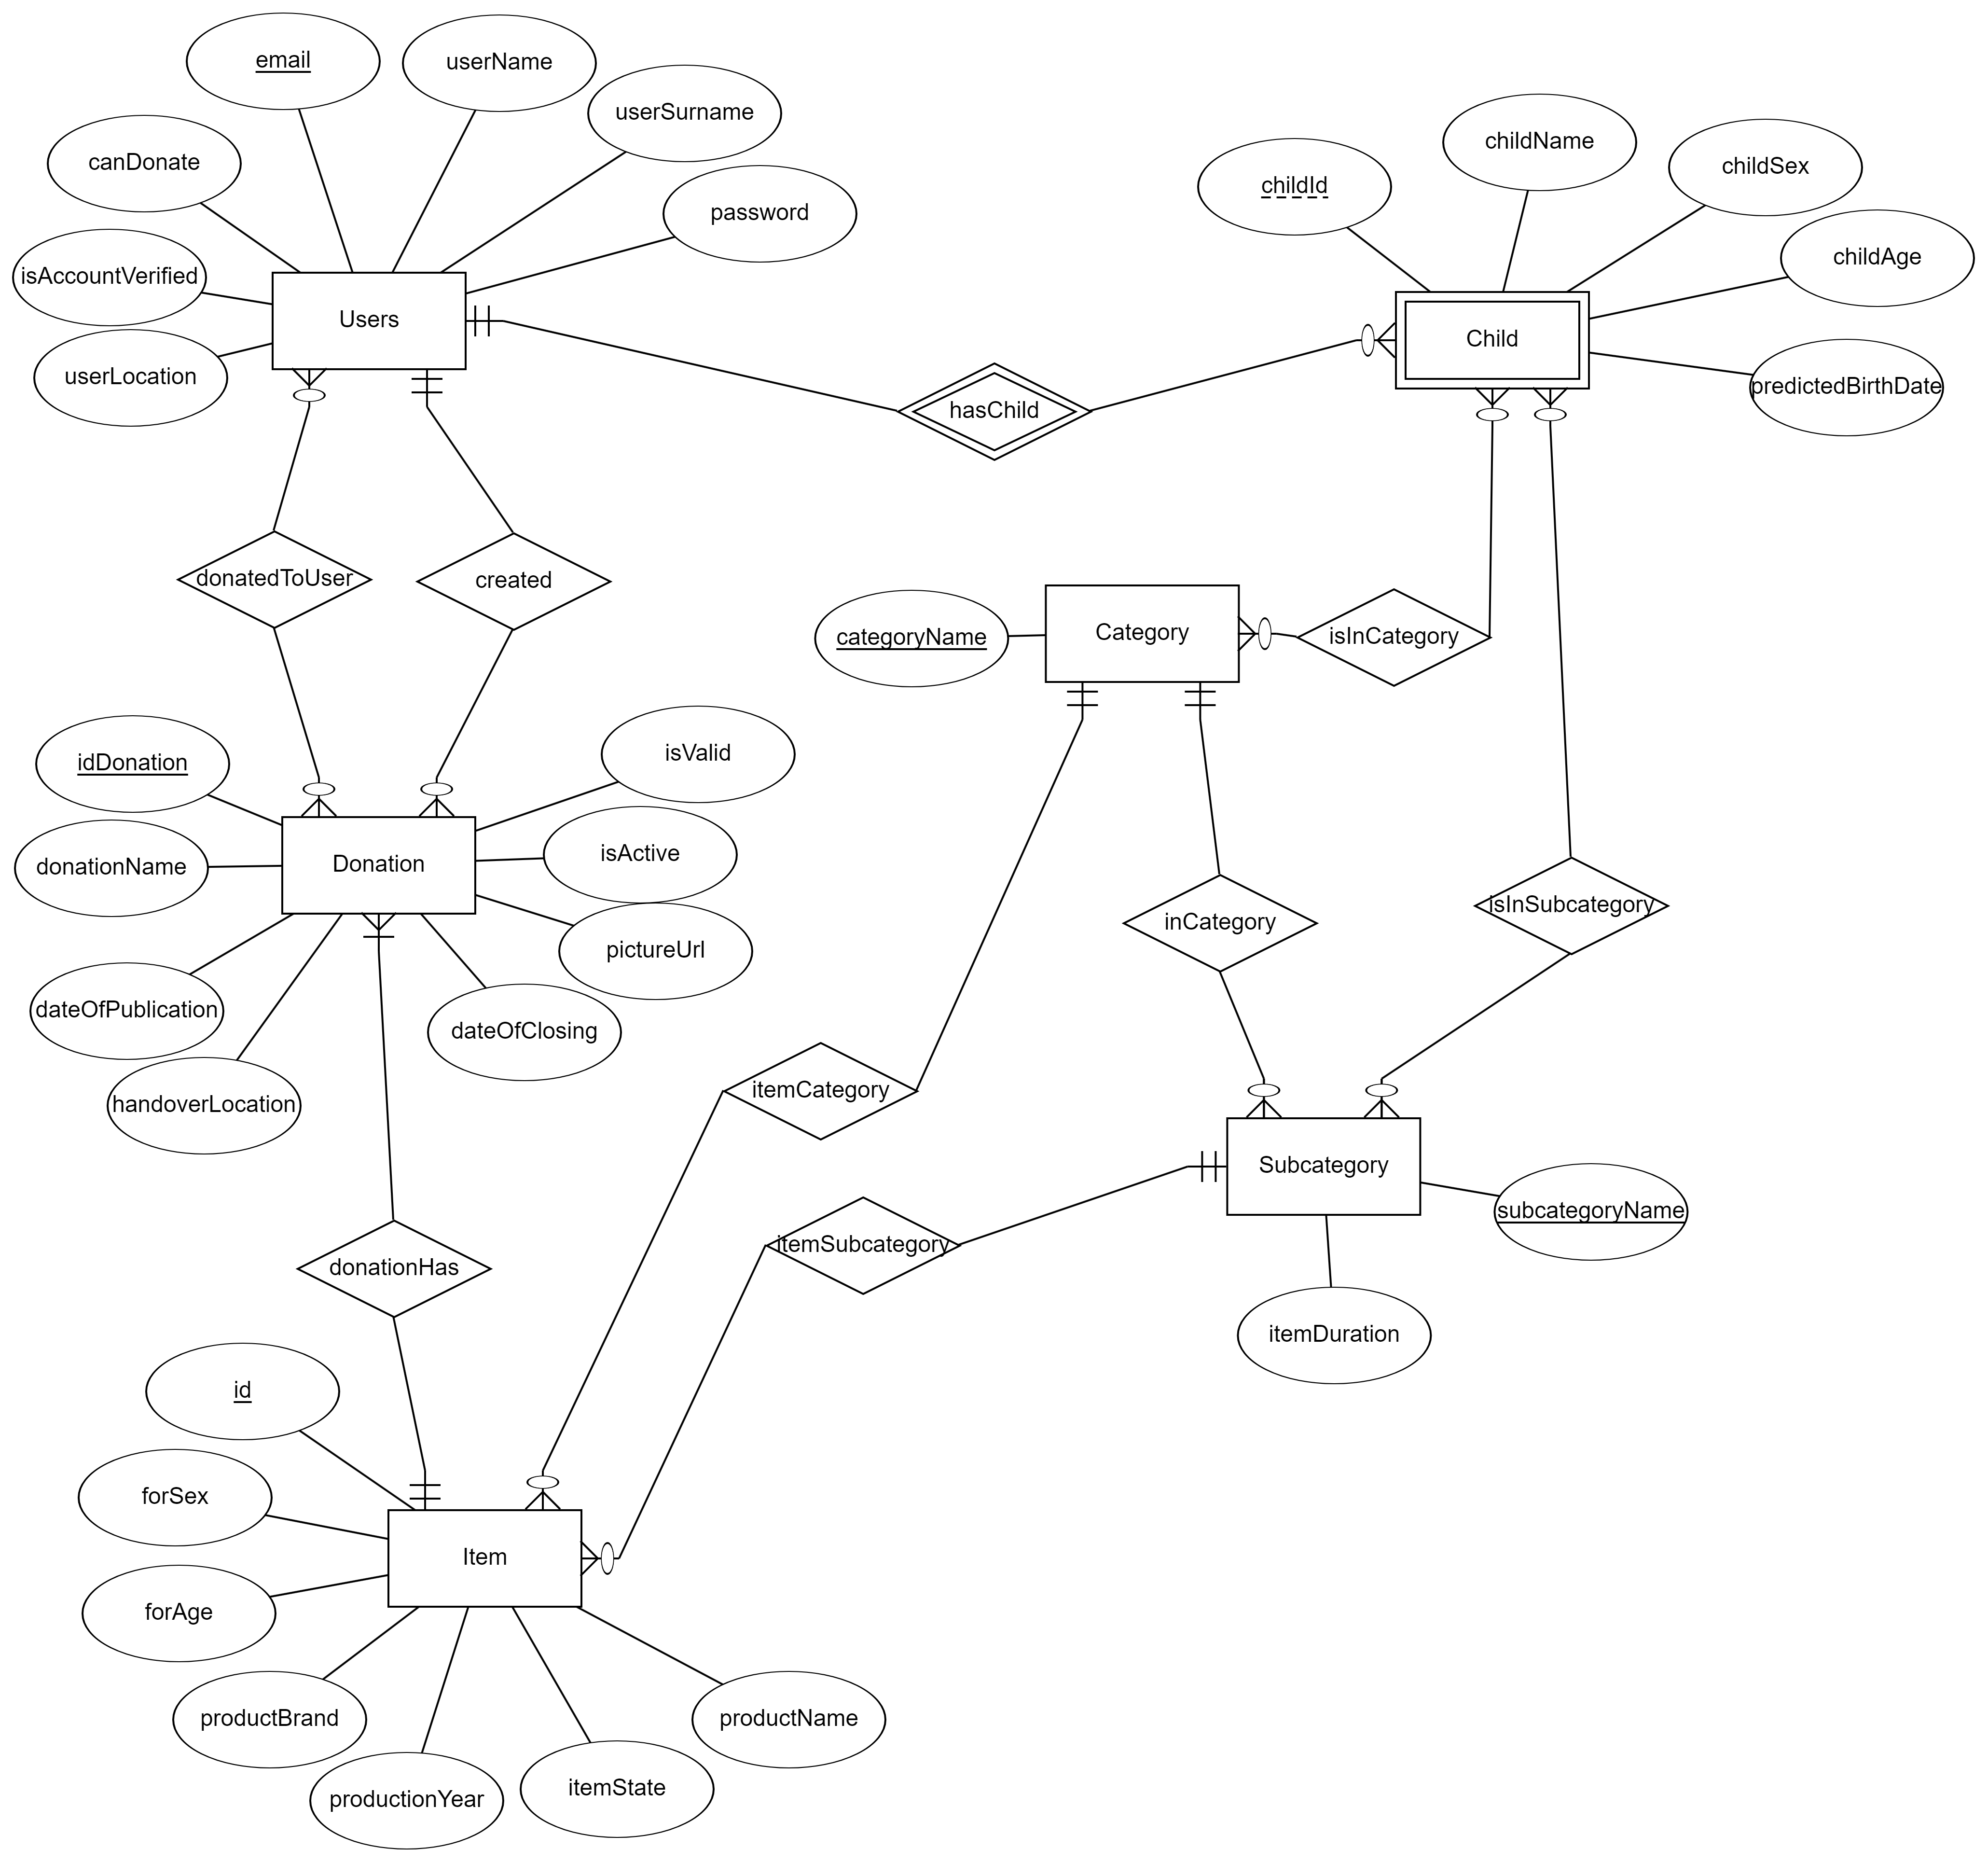
\includegraphics[width=\textwidth,height=0.7\textheight]{dijagrami/ERdijagram.png}
					\centering
					\caption{ER dijagram - aplikacija Djeca za djecu}
					\label{fig:ERDiagram}
				\end{figure}

				\begin{figure}[H]
					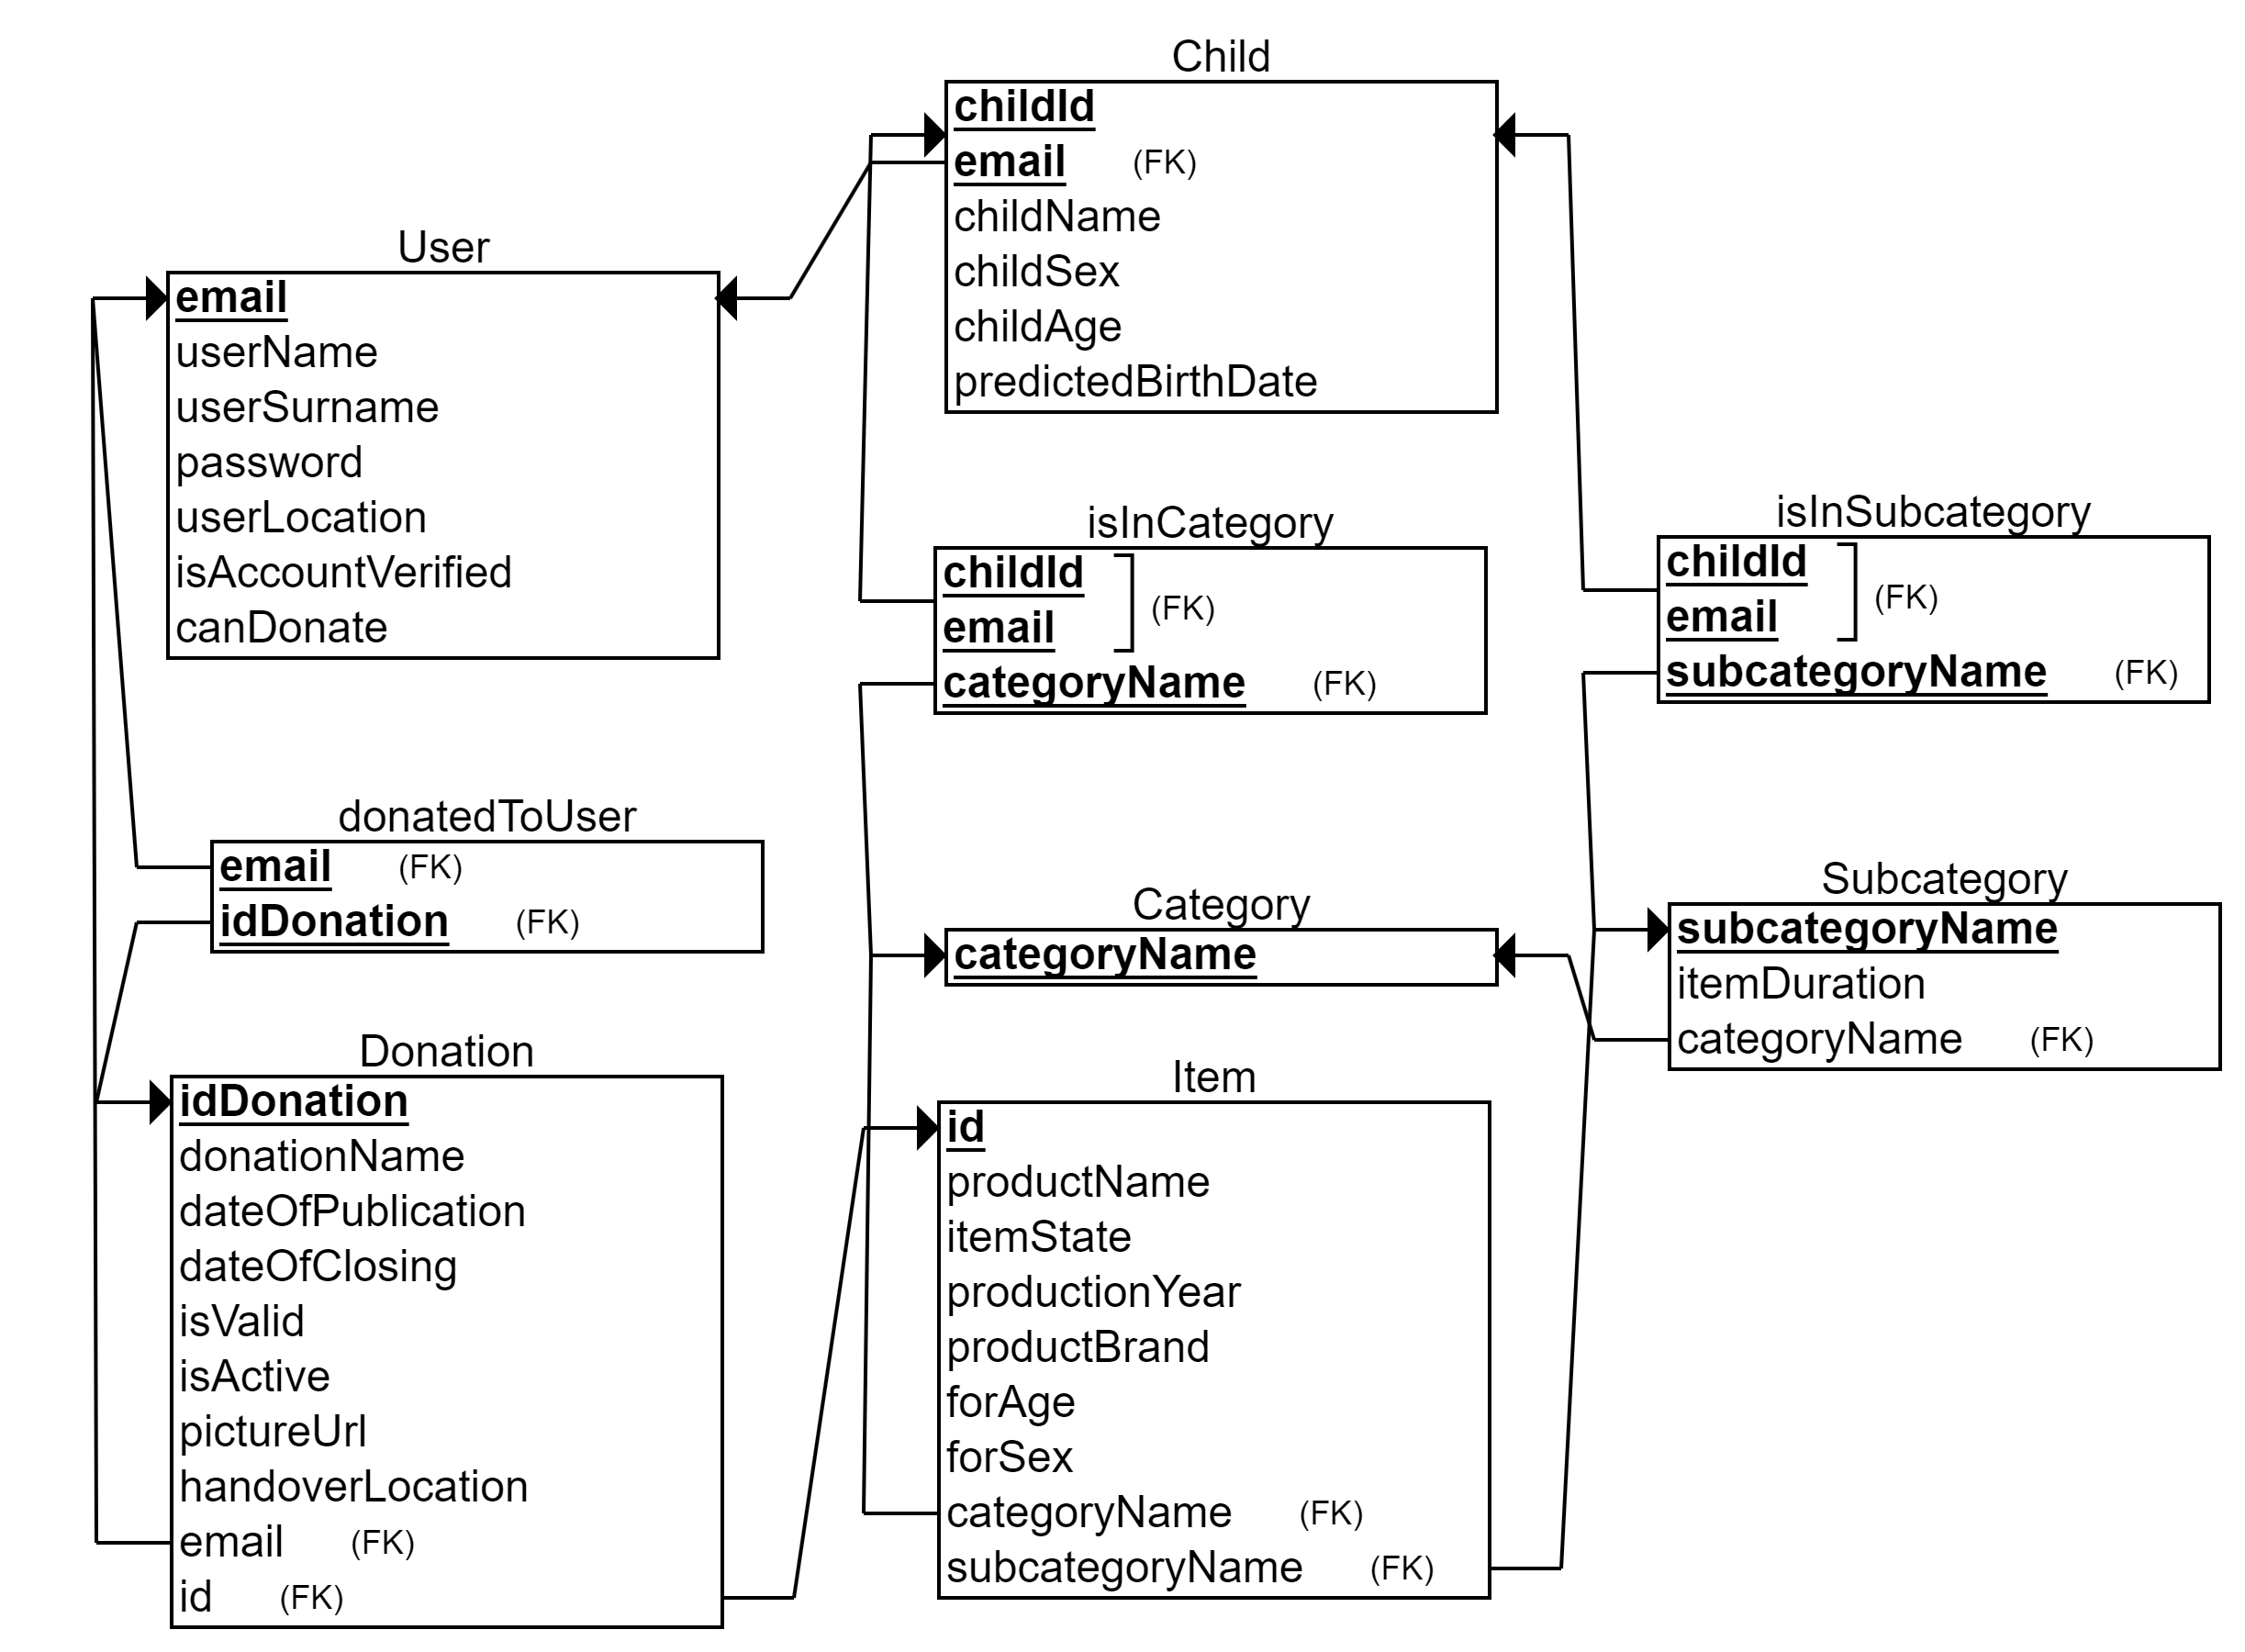
\includegraphics[width=\textwidth,height=0.7\textheight]{dijagrami/RelDijagram.png}
					\centering
					\caption{Relacijski dijagram - aplikacija Djeca za djecu}
					\label{fig:RelDijagram}
				\end{figure}
			\eject
			
			
		\section{Dijagram razreda}
			
			%\textbf{\textit{dio 1. revizije}}\\
			
			%\textit{Prilikom prve predaje projekta, potrebno je priložiti potpuno razrađen dijagram razreda vezan uz \textbf{generičku funkcionalnost} sustava. Ostale funkcionalnosti trebaju biti idejno razrađene u dijagramu sa sljedećim komponentama: nazivi razreda, nazivi metoda i vrste pristupa metodama (npr. javni, zaštićeni), nazivi atributa razreda, veze i odnosi između razreda.}\\
			
			Na slikama 4.4 do 4.7 prikazani su razredi koji pripadaju backend dijelu našeg sustava. U pitanju su specifikacijski dijagrami razreda - implementacijski dijagrami prikazani su nakon opisa specifikacijskih dijagrama.\\[5pt]

			Slika 4.4 prikazuje razrede koji predstavljaju modele - preslikane relacije baze podataka. Razred User predstavlja registriranog korisnika sustava. Razred Child predstavlja dijete registriranog korisnika sustava. Razred Donation predstavlja jednu donaciju zabilježenu u sustavu. 
			Razred Item predstavlja jedan predmet vezan za neke od donacija. Razred Category predstavlja podatke o jednoj od kategorija u koje mogu biti svrstani predmeti. Razred Subcategory predstavlja podatke o jednoj od potkategorija u koje mogu biti svrstani predmeti.\\[10pt]

			\begin{figure}[H]
				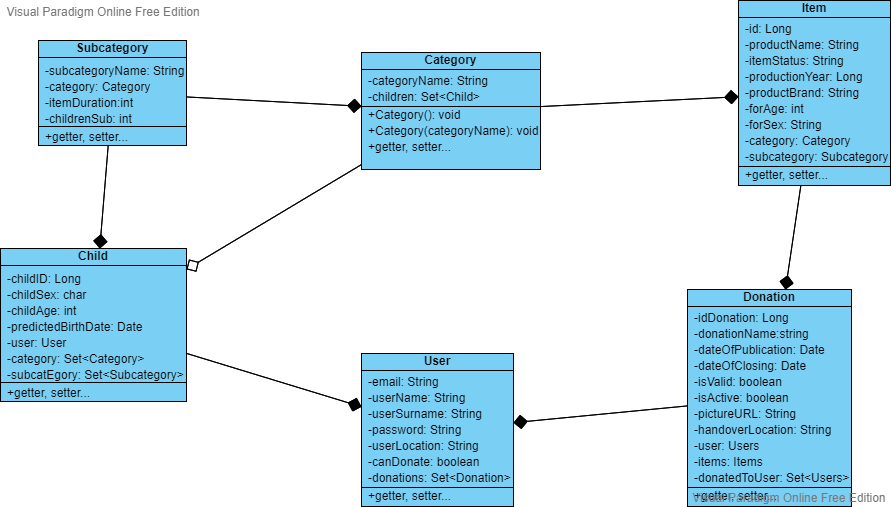
\includegraphics[width=\textwidth,height=0.35\textheight]{dijagrami/Modeli.png}
				\centering
				\caption{Dijagram razreda - dio Models}
				\label{fig:Models}
			\end{figure}
			\eject
			Slika 4.5 prikazuje odnos komponenti na primjeru razreda Category. Razred CategoryController prihvaća i odgovara na HTTP zahtjeve poslane od korisnika tj. konkretnije frontenda. Kako bi na njih ispravno odgovorio, uspostavlja komunikaciju s razredom CategoryServiceJpa.
			Razred CategoryServiceJpa implementira sučelje CategoryService kako bi obavljao potrebne izračune i osigurao uspješno provođenje poslovne logike. Uz to, razred CategoryServiceJpa uspostavlja komunikaciju s razredom CategoryRepository koji služi kao sučelje za pohranu i dohvat podataka iz baze.
			Kako bi prikaz bio što sažetiji, odnos komponenti prikazan je samo na jednom razredu. U stvarnoj implementaciji, ovakav odnos komponenti tj. razreda postoji za svaki razred iz dijela Models.\\[10pt]

			\begin{figure}[H]
				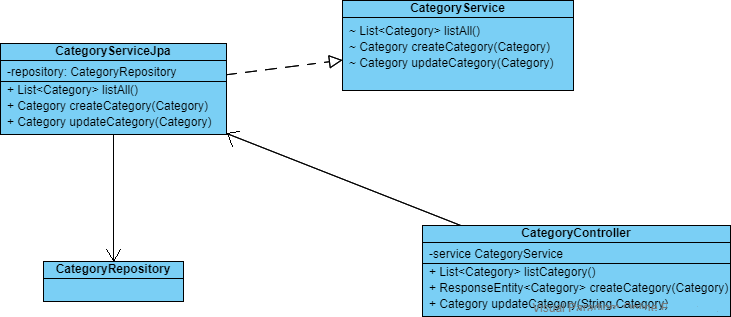
\includegraphics[width=\textwidth,height=0.35\textheight]{dijagrami/OdnosKomponenti.png}
				\centering
				\caption{Dijagram razreda - odnos komponenti}
				\label{fig:OdnosKomponenti}
			\end{figure}

			\eject

			Slika 4.6 prikazuje razrede izvedene iz razreda RestController. Svaki od razreda izvedenih iz RestController služi za prihvaćanje i odgovor na HTTP zahtjeve poslane od strane korisnika tj. konkretnije frontenda.\\[10pt]
			%Razred UsersController služi za slanje odgovora na zahtjeve vezane uz podatke o korisnicima.
			%Razred UsersDetailsService služi za slanje odgovora na zahtjeve vezane uz detaljne podatke o korisnicima.
			%Razred RolesController služi za slanje odgovora na zahtjev vezan uz podatke o ulogama korisnika.
			%Razred ChildController služi za slanje odgovora na zahtjeve vezane uz podatke o djeci.
			%Razred ItemController služi za slanje odgovora na zahtjeve vezane uz podatke o predmetima iz donacija.
			%Razred DonationController služi za slanje odgovora na zahtjeve vezane uz podatke o donacijama.
			%Razred CategoryController služi za slanje odgovora na zahtjeve vezane uz podatke o kategorijama.
			%Razred SubcategoryController služi za slanje odgovora na zahtjeve vezane uz podatke o potkategorijama.\\[10pt]

			\begin{figure}[H]
				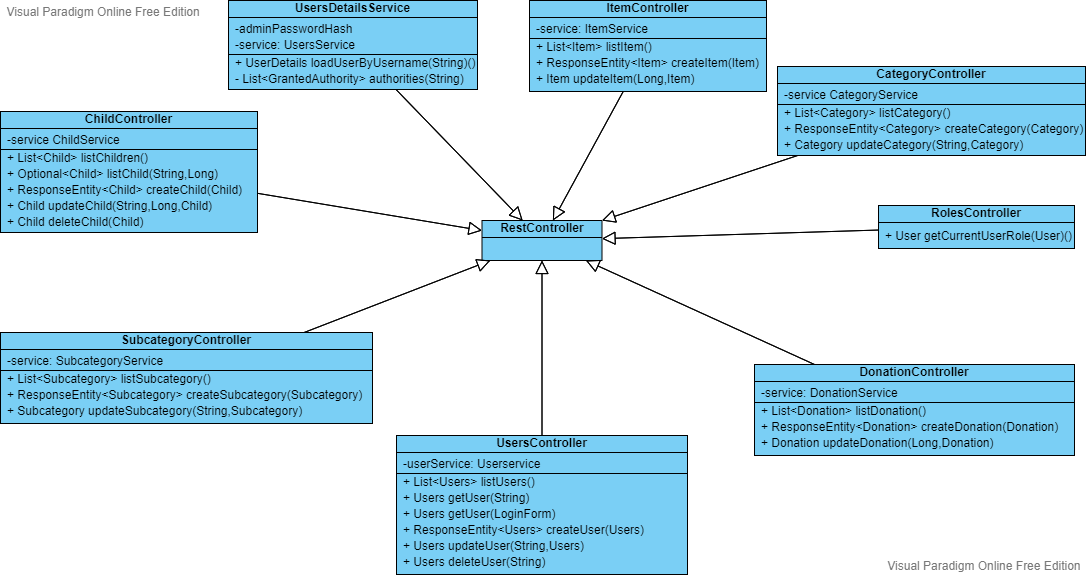
\includegraphics[width=\textwidth,height=0.4\textheight]{dijagrami/Controlleri.png}
				\centering
				\caption{Dijagram razreda - dio Controllers}
				\label{fig:Controllers}
			\end{figure}

			\eject

			Slika 4.7 prikazuje razrede izvedene iz razreda JpaRepository. Svaki od prikazanih razreda služi kao sučelje za pohranu i dohvat podataka iz baze podataka za svoju pripadajuću relaciju.\\[10pt]

			\begin{figure}[H]
				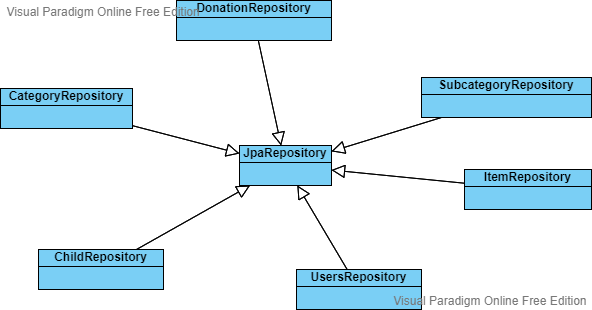
\includegraphics[width=\textwidth,height=0.4\textheight]{dijagrami/Repozitoriji.png}
				\centering
				\caption{Dijagram razreda - dio Repositories}
				\label{fig:Repositories}
			\end{figure}

			%\textbf{\textit{dio 2. revizije}}\\

                Na slikama 4.8 - 4.15 prikazani su implementacijski dijagrami razreda generirani direktno iz koda. Uz dijagrame razreda za koje su već opisani specifikacijski dijagrami (Models, odnos komponenti, Controllers, Repositories) dodatno su uključeni i dijagram razreda koji prikazuje odnos između UsersController klase i EmailSenderService klase koja se koristi za slanje potvrde o registraciji korisnika na mail, kao i dijagram razreda koji prikazuje odnos klasa za ostvarenje sigurnosti, autentifikacije i autorizacije korisnika. Zbog preglednosti dijagrami razreda za dio Controllers i dio Repositories podijeljeni su u dva dijela.
			
			\eject

                \begin{figure}[H]
				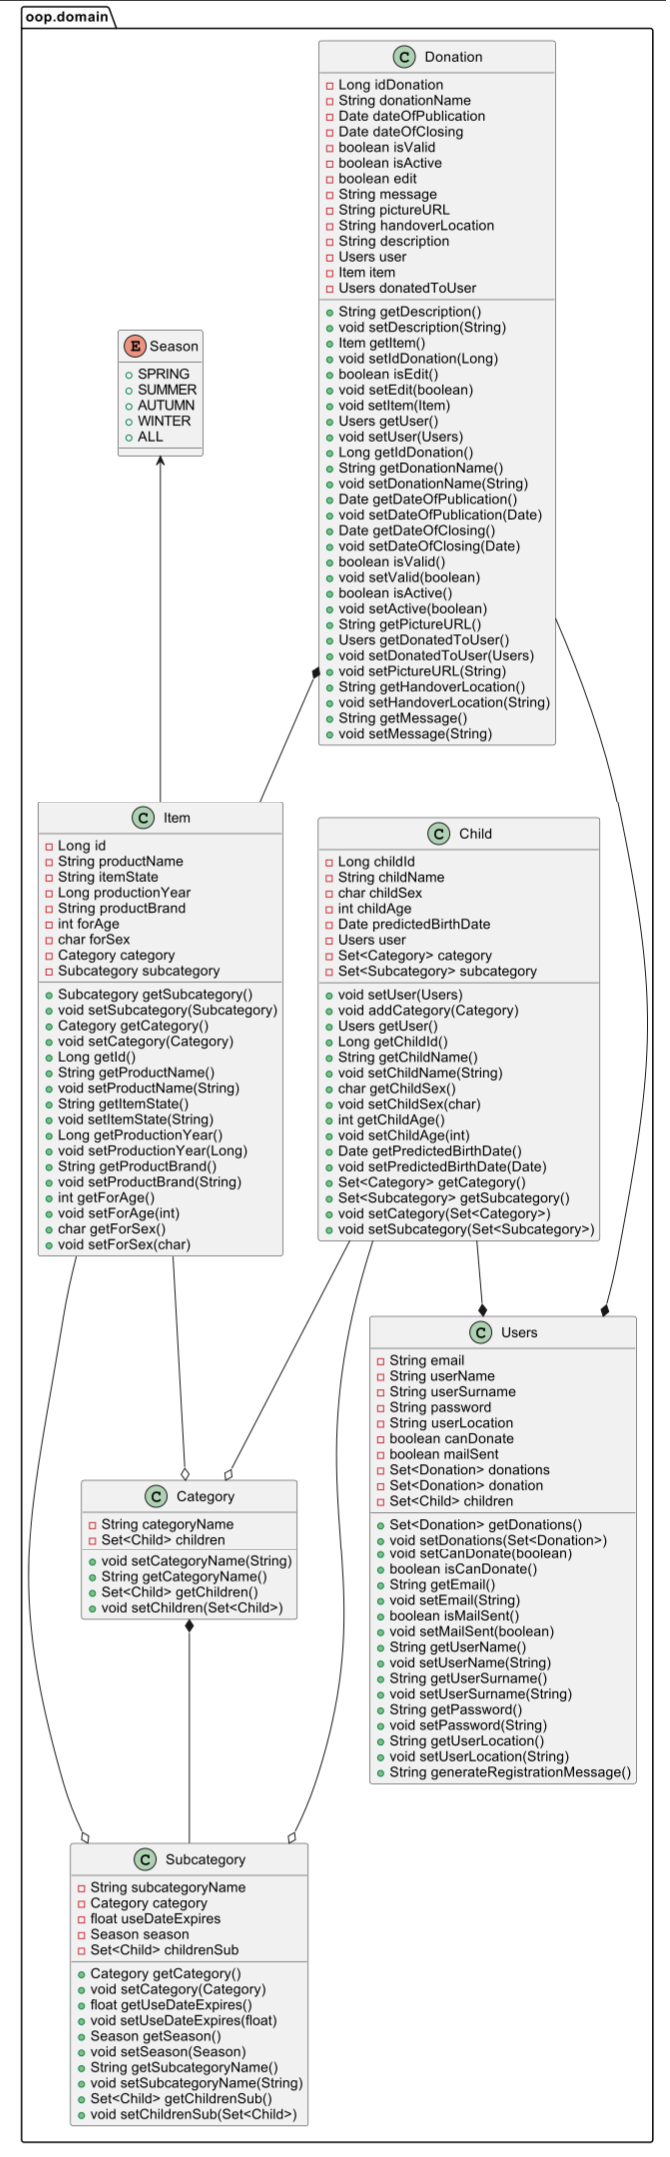
\includegraphics[width=\textwidth,height=0.95\textheight]{dijagrami/Modeli Final.png}
				\centering
				\caption{Dijagram razreda - dio Models (finalna verzija)}
				\label{fig:ModelsFinal}
			\end{figure}

                \begin{figure}[H]
				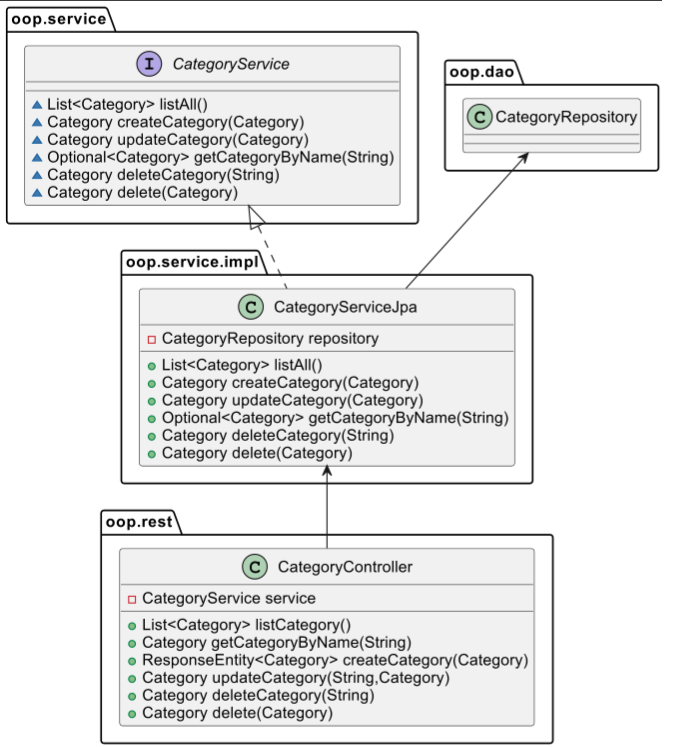
\includegraphics[width=\textwidth,height=0.8\textheight]{dijagrami/Odnos komponenti Final.png}
				\centering
				\caption{Dijagram razreda - odnos komponenti (finalna verzija)}
				\label{fig:OdnosKomponentiFinal}
			\end{figure}

                %   \begin{figure}[H]
                %   \makebox[\textwidth][c]{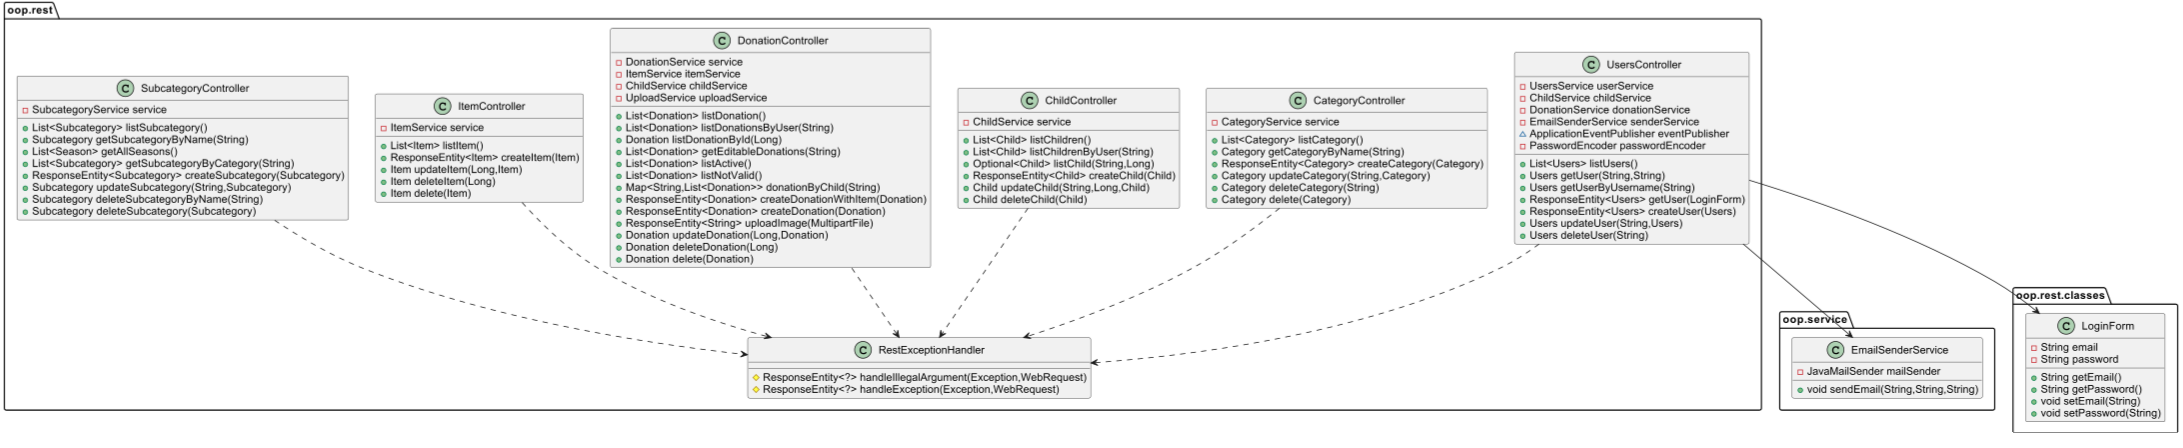
\includegraphics[width=1.3\textwidth,height=0.6\textheight]{dijagrami/Controlleri Final.png}}%
			% 	\centering
			% 	\caption{Dijagram razreda - dio Controllers (finalna verzija)}
			% 	\label{fig:ControllersFinal}
			% \end{figure}

                \begin{figure}[H]
				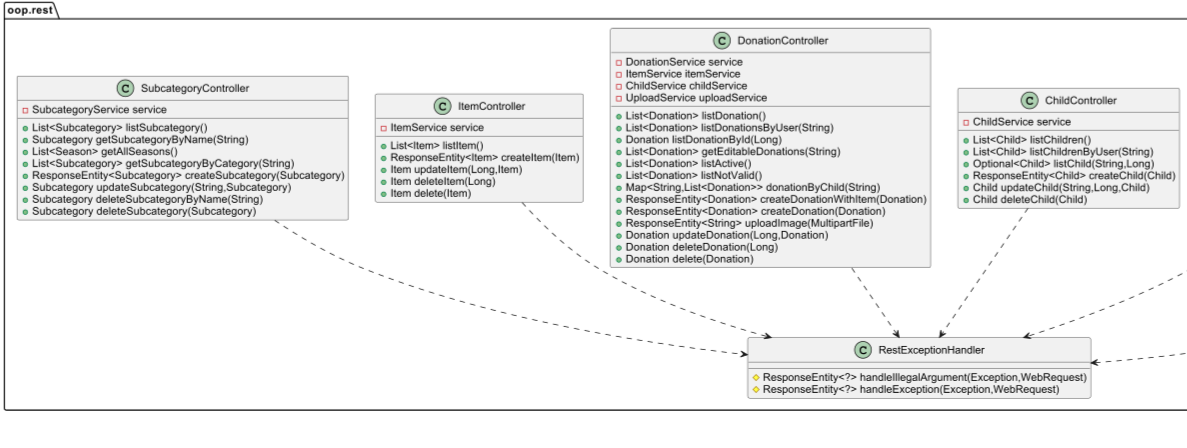
\includegraphics[width=\textwidth,height=0.4\textheight]{dijagrami/Controlleri Final Part1.png}
				\centering
				\caption{Dijagram razreda - dio Controllers, prvi dio (finalna verzija)}
				\label{fig:ControllersFinalPt1}
			\end{figure}

                \begin{figure}[H]
				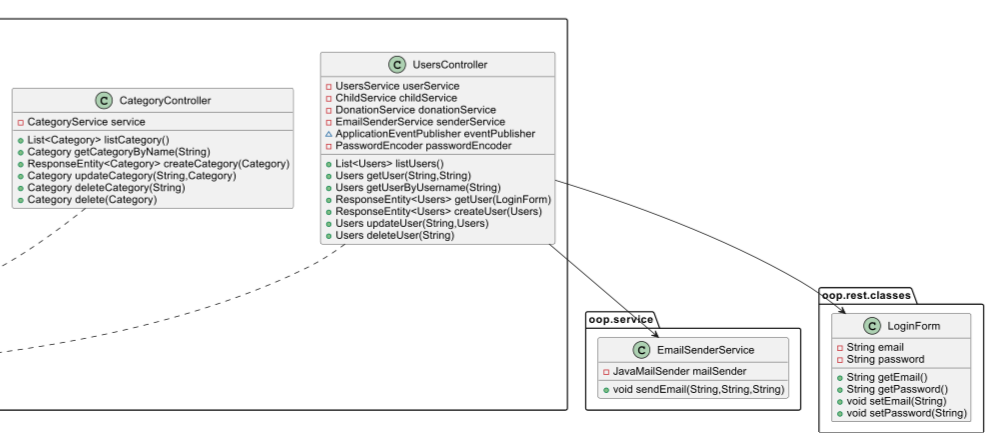
\includegraphics[width=\textwidth,height=0.4\textheight]{dijagrami/Controlleri Final Part2.png}
				\centering
				\caption{Dijagram razreda - dio Controllers, drugi dio (finalna verzija)}
				\label{fig:ControllersFinalPt2}
			\end{figure}

                \begin{figure}[H]
                \makebox[\textwidth][c]{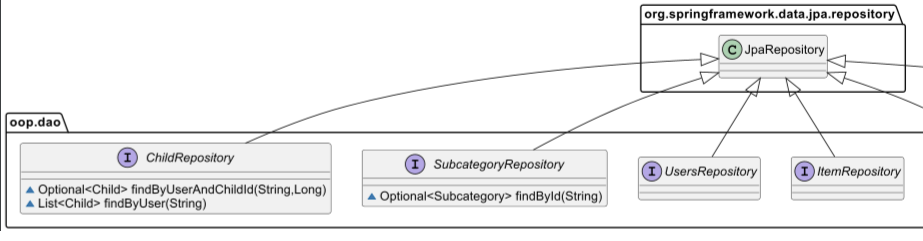
\includegraphics[width=1.2\textwidth,height=0.4\textheight]{dijagrami/Repozitoriji Final Part1.png}}%
				\centering
				\caption{Dijagram razreda - dio Repositories, prvi dio (finalna verzija)}
				\label{fig:RepositoriesFinalPt1}
			\end{figure}

                \begin{figure}[H]
				\makebox[\textwidth][c]{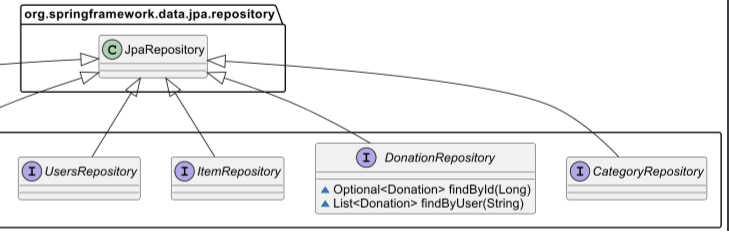
\includegraphics[width=1.2\textwidth,height=0.4\textheight]{dijagrami/Repozitoriji Final Part2.png}}%
				\centering
				\caption{Dijagram razreda - dio Repositories, drugi dio (finalna verzija)}
				\label{fig:RepositoriesFinalPt2}
			\end{figure}

                \begin{figure}[H]
				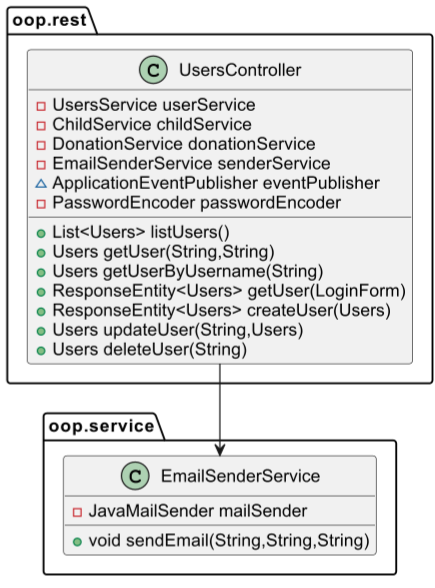
\includegraphics[width=\textwidth,height=0.4\textheight]{dijagrami/EmailService.png}
				\centering
				\caption{Dijagram razreda - dio Email Service}
				\label{fig:EmailService}
			\end{figure}

                \begin{figure}[H]
				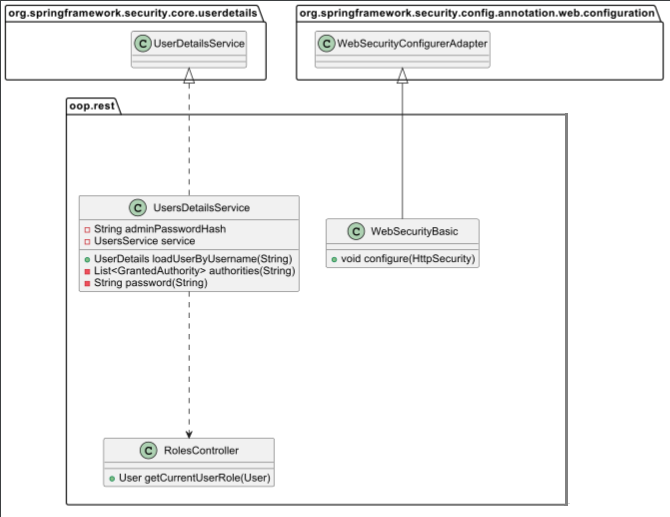
\includegraphics[width=\textwidth,height=0.4\textheight]{dijagrami/Security.png}
				\centering
				\caption{Dijagram razreda - dio Security}
				\label{fig:Security}
			\end{figure}
   
			\eject
		
		\section{Dijagram stanja}
			
                Dijagram stanja prikazan na slici 4.16 prikazuje stanja u kojima se može naći sustav (konkretno, u pitanju je korisničko sučelje - frontend), kao i prijelaze pomoću kojih sustav dolazi u druga stanja. Svaki prijelaz označen je događajem (npr. "Klik na proizvoljni oglas"), kao i akcijom (npr. "Prikaži aktivne oglase()") koja se izvršava "tijekom prijelaza" - nakon što se dogodio događaj koji je potaknuo prijelaz u drugo stanje. Većina akcija označenih na prijelazima isto tako mogla je biti označena kao entry odnosno exit akcija samoga stanja, ali je zbog preglednosti i konzistentnosti odabran prikaz takvih akcija na prijelazima. Dijagram na slici 4.16 prikazuje stanja u kojima se sustav može naći kada je u sustav ulogiran registrirani korisnik za kojeg je administrator stavio dopuštenje da može donirati - da korisnik nema dopuštenje, sustav se pri radu s takvim korisnikom ne bi mogao naći u stanju "Kreiranje oglasa", kao ni u stanju "Korisnikove donacije" jer ono služi za prikaz korisnikovih prijašnjih, kao i trenutnih donacija. \\

                \begin{figure}[H]
				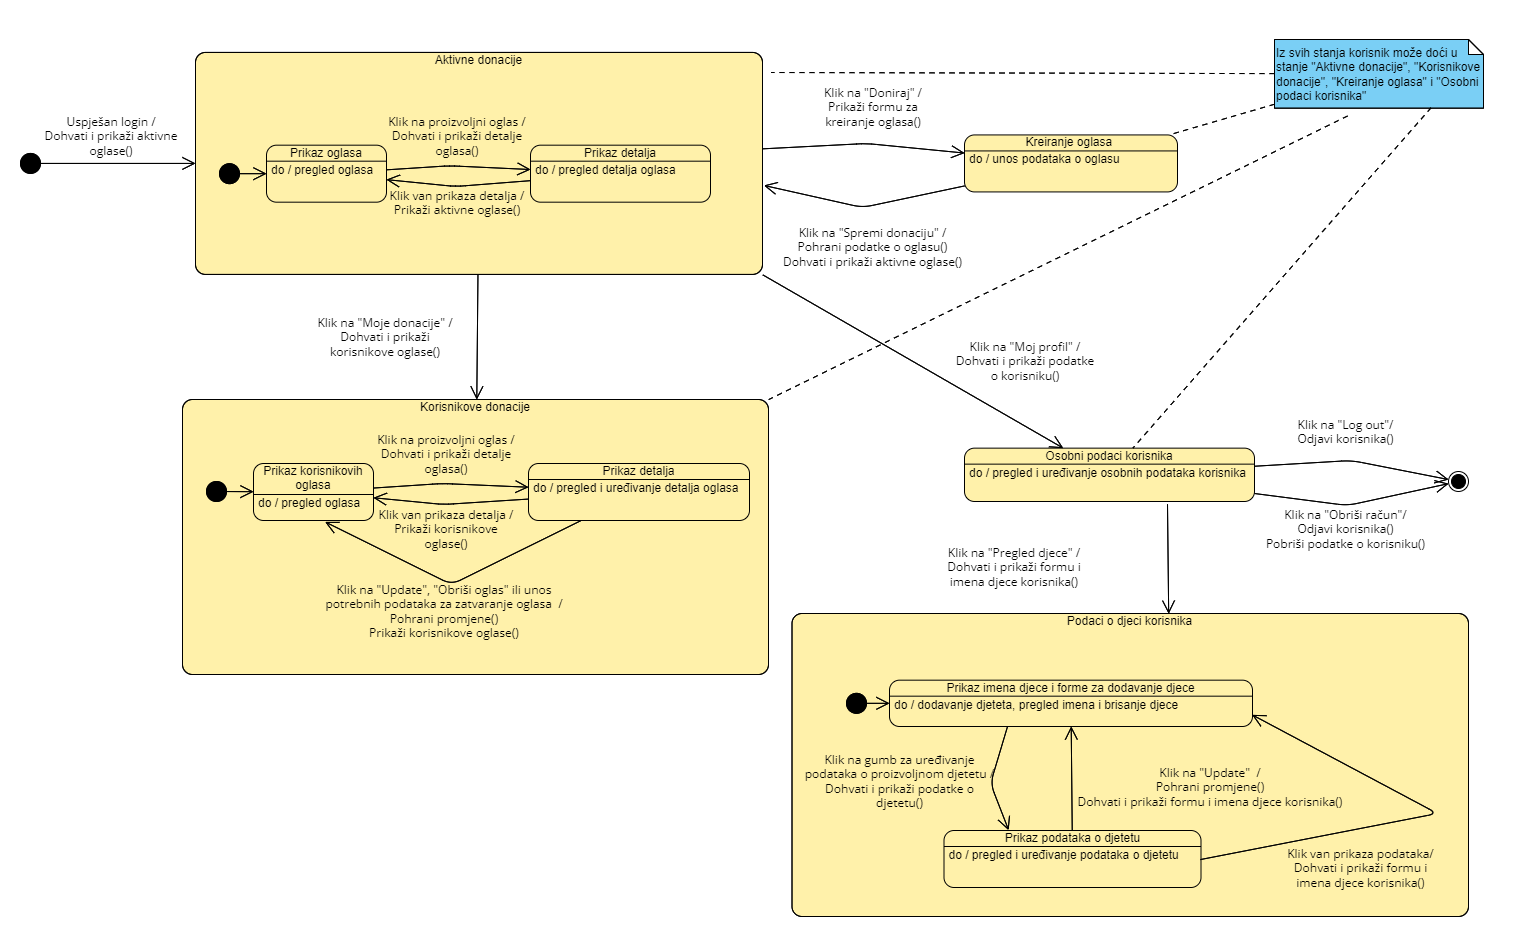
\includegraphics[width=\textwidth,height=0.45\textheight]{dijagrami/Dijagram stanja.png}
				\centering
				\caption{Dijagram stanja}
				\label{fig:StateDiagram}
			\end{figure}
			
			\eject 
                
                Kako bi napravili razliku između akcija koje izvršava sustav i akcija koje radi korisnik u interakciji sa sustavom, sve akcije koje izvršava sustav na kraju imaju oznaku () (slično pozivu funkcije u kodu). Radi preglednosti, neke od strelica nisu prikazane na dijagramu - korisnik iz bilo kojeg stanja može preći u stanje "Aktivne donacije", "Korisnikove donacije", "Kreiranje oglasa" i "Osobno podaci korisnika" jer je prijelaz u ta stanja ostvaren klikom na odgovarajući dio zaglavlja stranice. Akcije koje radi korisnik u interakciji u sustavu naznačene su kao do akcije unutar stanja ili kao događaji koji potiču prijelaze u druga stanja.\\
                                
			Nakon uspješnog logina, registrirani korisnik preusmjeren je na stranicu Aktivne donacije na kojoj može pregledavati sve oglase, ali isto tako i pregledavati detalje proizvoljnih oglasa. Pomoću zaglavlja stranice korisnik može doći do stranice Aktivne donacije, stranice za kreiranje oglasa, stranice za prikaz i uređivanje osobnih podataka te stranice za prikaz vlastitih donacija. Na stranici za kreiranje oglasa korisnik unosi podatke i nakon unosa klikom na gumb "Spremi donaciju" biva preusmjeren na stranicu za prikaz vlastitih donacija. Na stranici za prikaz vlastitih donacija korisnik može pregledavati sve oglase koje je sam kreirao ili zaprimio, kao i detalje o istima. Na stranici za prikaz i uređivanje osobnih podataka korisnik se također može i odjaviti, obrisati svoj račun i otići na stranicu za dodavanje, brisanje i prikaz podataka o djeci. Rad s aplikacijom završava kada korisnik odabere opciju "Log out".
			%\textbf{\textit{dio 2. revizije}}\\

                \eject
                %\textbf{V2}

                %Dijagram stanja prikazan na slici 4.9 prikazuje stanja u kojima se može naći sustav (konkretno, u pitanju je korisničko sučelje - frontend), kao i prijelaze pomoću kojih sustav dolazi u druga stanja. Svaki prijelaz označen je događajem (npr. "Klik na proizvoljni oglas"), a po potrebi i uvjetom (u uglatim zagradama). \\

                %\begin{figure}[H]
                %\makebox[\textwidth][c]{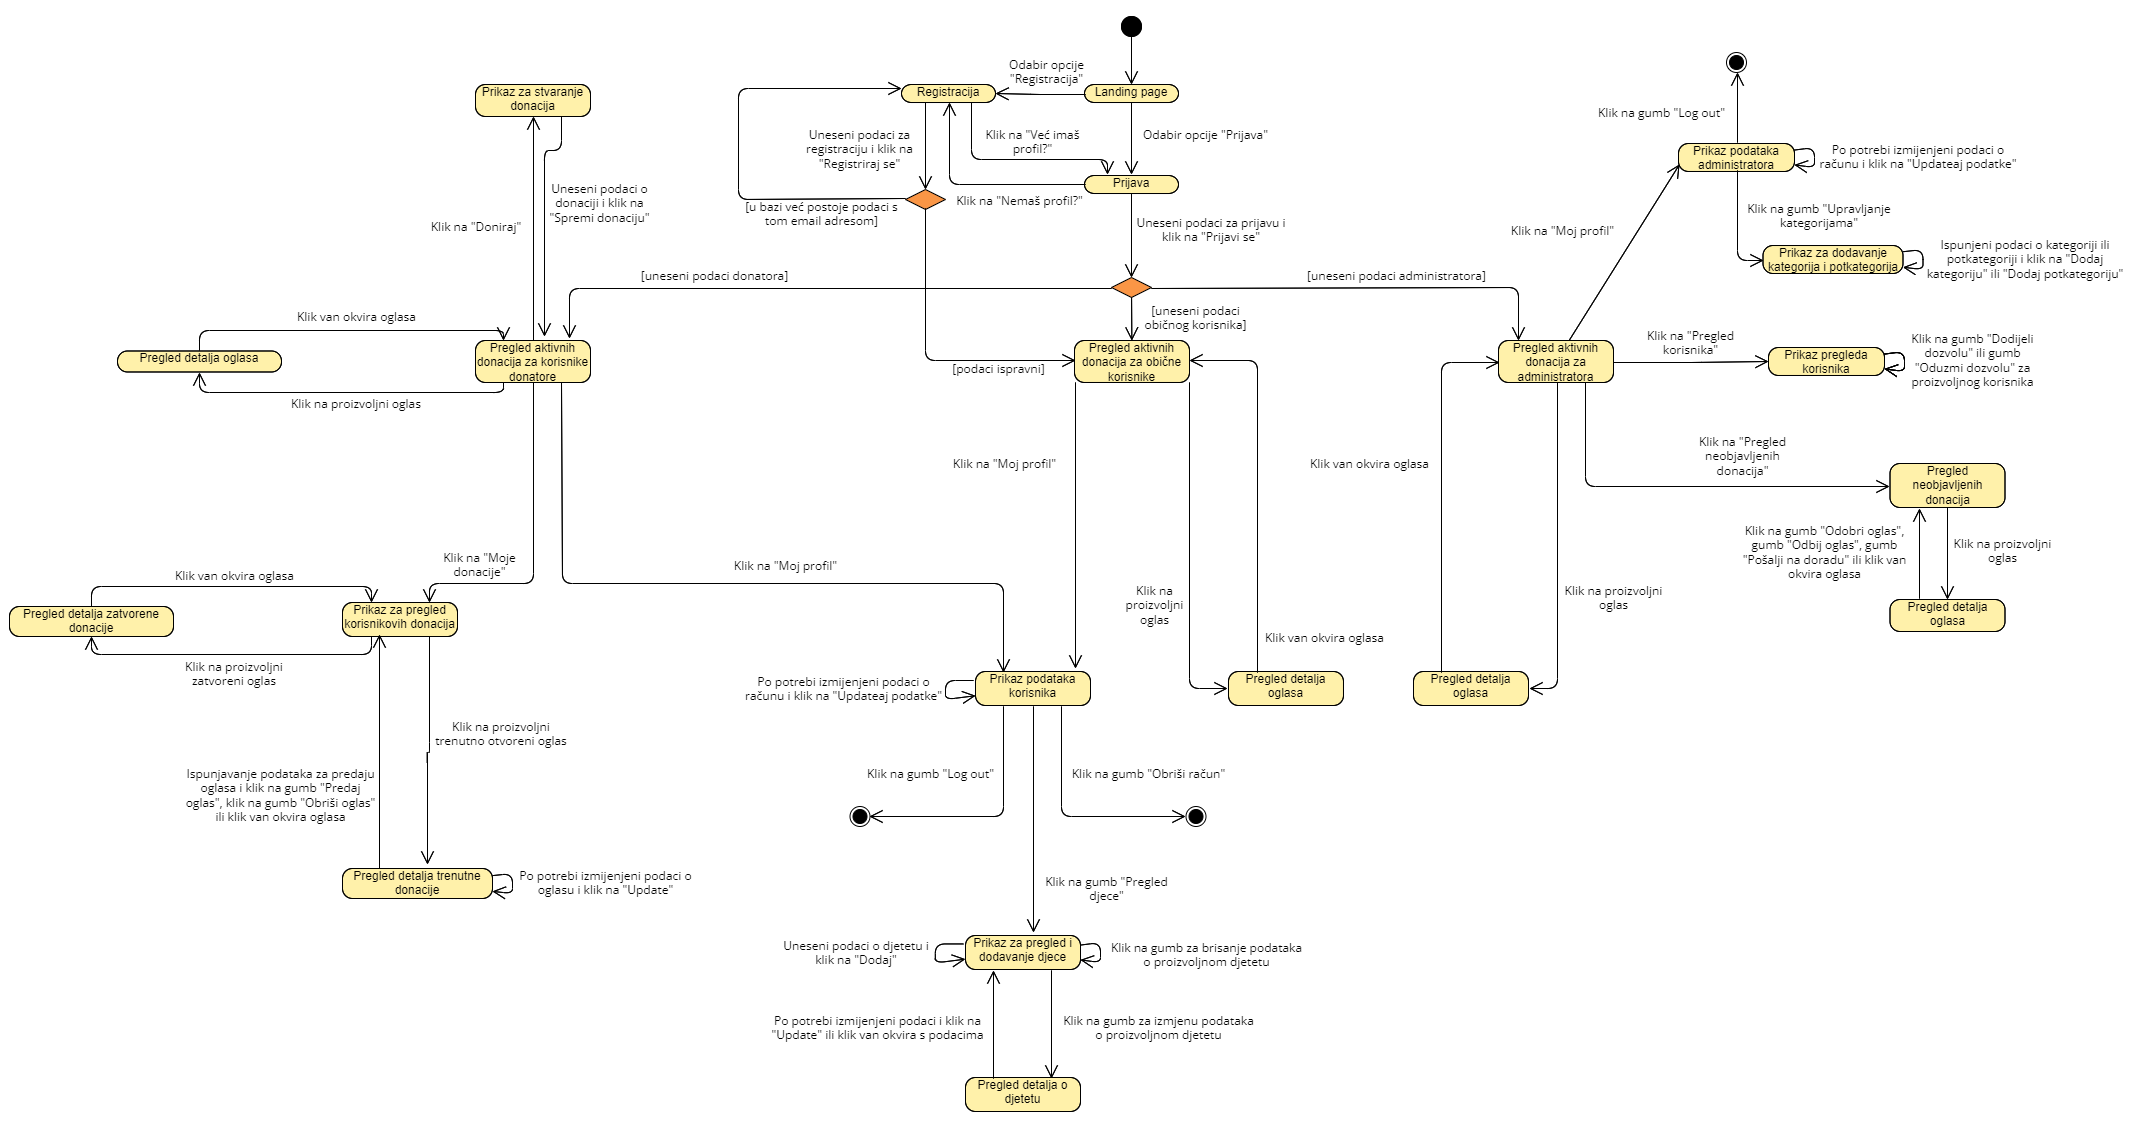
\includegraphics[scale=0.35]{dijagrami/Dijagram stanja v2.png}}%
				%\centering
				%\caption{Dijagram stanja, druga inačica}
				%\label{fig:StateDiagramv2}
			%\end{figure}
                 %Ovisno o tome koja je razina prava dodijeljena korisniku s unešenim podacima, nakon uspješnog logina korisniku se prikaže jedna od tri moguće stranice. Stranice se razlikuju u izgledu svoga zaglavlja (engl. page header) - administrator ima opcije pregledavati aktivne oglase, pregledavati i odobravati neobjavljene oglase, pregledavati popis korisnika i dodijeljivati im pravo za doniranje, ali i pregledavati i mijenjati svoje podatke. S druge strane, običan korisnik ima pravo samo pregledavati aktivne oglase i pregledavati i mijenjati vlastite podatke, pritom dodajući, brišući ili izmjenjujući podatke o svojoj djeci. Donator uz mogućnosti običnog korisnika može i stvarati oglase te pregledavati svoje do sada objavljene oglase, bilo da je u pitanju već zatvoren oglas ili trenutno otvoreni oglas - trenutno otvorene oglase donatori mogu urediti, obrisati ili zatvoriti. \\
                 
                 %Radi preglednosti, neke od strelica nisu prikazane na dijagramu - običan korisnik iz bilo kojeg stanja može preći u stanje "Prikaz aktivnih donacija za obične korisnike" i  "Prikaz podataka korisnika". Donator uz prijelaz u navedena stanja ("Pregled aktivnih donacija za korisnike donatore", "Prikaz podataka korisnika") može iz bilo kojeg stanja prijeći i u stanja "Prikaz za pregled korisnikovih donacija" i "Prikaz za stvaranja donacija", a administrator može iz bilo kojeg stanja prijeći u jedno od sljedećih stanja: "Pregled aktivnih donacija za administratora", "Prikaz podataka administratora", "Prikaz pregleda korisnika", "Pregled neobjavljenih donacija" i "Pregled aktivnih donacija za administratora". Prijelazi u stanja navedena u ovome odlomku ostvareni su klikom na prikladne dijelove zaglavlja stranice, a sama zaglavlja razlikuju se ovisno o razini ovlasti korisnika.\\

                 %Radi preglednosti, nakon klika na gumb "Log out" ili "Obriši račun" sustav ide u završno stanje - u stvarnosti time samo završava trenutna sesija korištenja sustava te se korisniku prikazuje landing page, ali bi dodavanjem strelica za prijelaz u stanje "Landing page" iz potrebnih stanja bila narušena preglednost dijagrama. Akcije sustava (npr. prikaziOglase()) zbog preglednosti također su izostavljena iz dijagrama, time na dijagramu ostavljajući samo korisničke akcije kao događaje koji potiču prijelaz iz jednog stanja sustava u drugo. Isto tako, provjere ispravnosti podataka (npr. provjera jesu li izmijenjeni podaci o korisniku i dalje važeći) izostavljene su iz dijagrama - za svaku provjeru bilo bi potrebno uvesti grananje gdje bi ovisno o ispravnosti podataka sustav ponovno došao u prethodno stanje ili mogao dalje napredovati. 

                %\eject
		
		%\section{Dijagram aktivnosti}
			
			%\textbf{\textit{dio 2. revizije}}\\
			
			 %\textit{Potrebno je priložiti dijagram aktivnosti s pripadajućim opisom. Dijagram aktivnosti treba prikazivati značajan dio sustava.}
			
			%\eject
		%\section{Dijagram komponenti}
		
			%\textbf{\textit{dio 2. revizije}}\\
		
			% \textit{Potrebno je priložiti dijagram komponenti s pripadajućim opisom. Dijagram komponenti treba prikazivati strukturu cijele aplikacije.}
	\chapter{Implementacija i korisničko sučelje}
		
		
		\section{Korištene tehnologije i alati}
		
			%\textbf{\textit{dio 2. revizije}}
			Kako bi što više ubrzali i olakšali komunikaciju među članovima tima, koristili smo dvije aplikacije: \underline{Whatsapp}\footnote{\url{https://www.whatsapp.com/}} i \underline{Discord}\footnote{\url{https://discord.com/}}. Kako bismo se dodatno upoznali s tehnologijom koja se često koristi u praksi, koristili smo i platformu \underline{Jira}\footnote{\url{https://www.atlassian.com/software/jira}} za organizaciju i podjelu zadataka na članove tima putem zadataka (engl. task) na Kanban ploči. Kao distribuirani sustav za upravljanje izvornim kodom koristili smo \underline{Git}\footnote{\url{https://git-scm.com/}}, a sami repozitorij projekta dostupan je na platformi \underline{Gitlab}\footnote{\url{https://gitlab.com/}}\\

            Za razvoj korisničkog sučelja tj. frontenda općenito, korišteni su markup jezik \underline{HTML}\footnote{\url{https://en.wikipedia.org/wiki/HTML}}, stilski jezik \underline{CSS}\footnote{\url{https://en.wikipedia.org/wiki/CSS}}, programski jezik \underline{Javascript}\footnote{\url{https://www.javascript.com/}} i \underline{React.js}\footnote{\url{https://reactjs.org/}}. React.js knjižnica je pisana u jeziku Javascript koja omogućava jednostavan i relativno brz razvoj komponenti koje je lako ponovno koristiti, a razvija ga primarno tvrtka Meta. Uz React.js, za razvoj robusnih i kvalitetnih komponenti, korišten je \underline{Material UI}\footnote{\url{https://mui.com/}} - open-source knjižnica React komponenti. Za pisanje koda u navedenim jezicima korišten je \underline{Visual Studio Code}\footnote{\url{https://code.visualstudio.com/}} - veoma popularan IDE (integrirana razvojna okolina) s velikim brojem opcionalnih ekstenzija koje služe kao pomoć pri razvoju. VSC razvija tvrtka Microsoft. \\

            \eject

            Za razvoj backenda korišten je programski jezik \underline{Java}\footnote{\url{https://www.java.com/en/}} - objektno orijentirani jezik korišten u brojnim aspektima razvoja programske potpore. Jezik Java razvija tvrtka Oracle. Uz to, korišten je \underline{Java Spring Boot}\footnote{\url{https://spring.io/projects/spring-boot}} - specijalizacija radnog okvira \underline{Java Spring}\footnote{\url{https://spring.io/}} razvijena s ciljem što bržeg, lakšeg i učinkovitijeg razvoja web aplikacija. Za pisanje koda u jeziku Java korišten je \underline{IntelliJ IDEA}\footnote{\url{https://www.jetbrains.com/idea/}} - integrirana razvojna okolina često korištena za razvoj programske potpore u jezicima Java i Kotlin. Intellij IDEA razvija tvrtka JetBrains. \\

            Za razvoj baze podataka korišten je sustav za upravljanje relacijskim bazama podataka \underline{PostgreSQL}\footnote{\url{https://www.postgresql.org/}}. Uz to, za lokalni razvoj i testiranje baze podataka korištena je aplikacija \underline{pgAdmin}\footnote{\url{https://www.pgadmin.org/}}. \\

            Za kreiranje potrebnih UML dijagrama korišten je alat \underline{Visual Paradigm Online}\footnote{\url{https://online.visual-paradigm.com/}} koji omogućava zajednički rad na dijagramima, time olakšavajući organizaciju i dijeljenje istih s članovima tima. Za razvoj dokumentacije korišten je markup jezik \underline{LaTeX}\footnote{\url{https://www.latex-project.org/}}, već navedena integrirana razvojna okolina Visual Studio Code i alat \underline{Overleaf}\footnote{\url{https://www.overleaf.com/}} koji omogućava online pisanje LaTeX koda.\\

            Frontend, backend i baza podataka pušteni su u pogon na platformi \underline{Render}\footnote{\url{https://render.com/}} koja omogućava besplatan i relativno jednostavan deploy aplikacija. Za uspješno puštanje u pogon backend koda, potrebno je pripremiti i \underline{Docker}\footnote{\url{https://www.docker.com/}} Container kako bi na istom mjestu bilo dostupno sve potrebno za uspješno puštanje backend-a u pogon. \\
		
			\eject 
		
	
		\section{Ispitivanje programskog rješenja}
			
			%\textbf{\textit{dio 2. revizije}}\\
			
			 Kako bismo što učinkovitije testirali naš sustav, testirali smo ispravnost rada pojedinih komponenti koristeći unit testove, ali i ispravnost rada čitavog sustava koristeći alat Selenium.
	
			
			\subsection{Ispitivanje komponenti}

                Za testiranje rada komponenti, napisano je i pokrenuto 9 unit testova. Testovi su pisani u programskom jeziku Java koristeći okvir za testiranje JUnit. Na slikama se nalazi kod samih testova, kao i dokaz da testovi prolaze (redak Tests passed). Uz to, vidljivo je i trajanje izvođenja testova.\\
                
                \subsubsection{Test 1}
                Prvim testom provjerava se valjanost zapisa o kategoriji pri dohvaćanju potkategorije - ako je dohvaćena potkategorija "Lutke", u dohvaćenom podatku trebao bi postojati i zapis o pripadnoj kategoriji - "Igračke". \underline{Test prolazi.}

                \begin{figure}[H]
				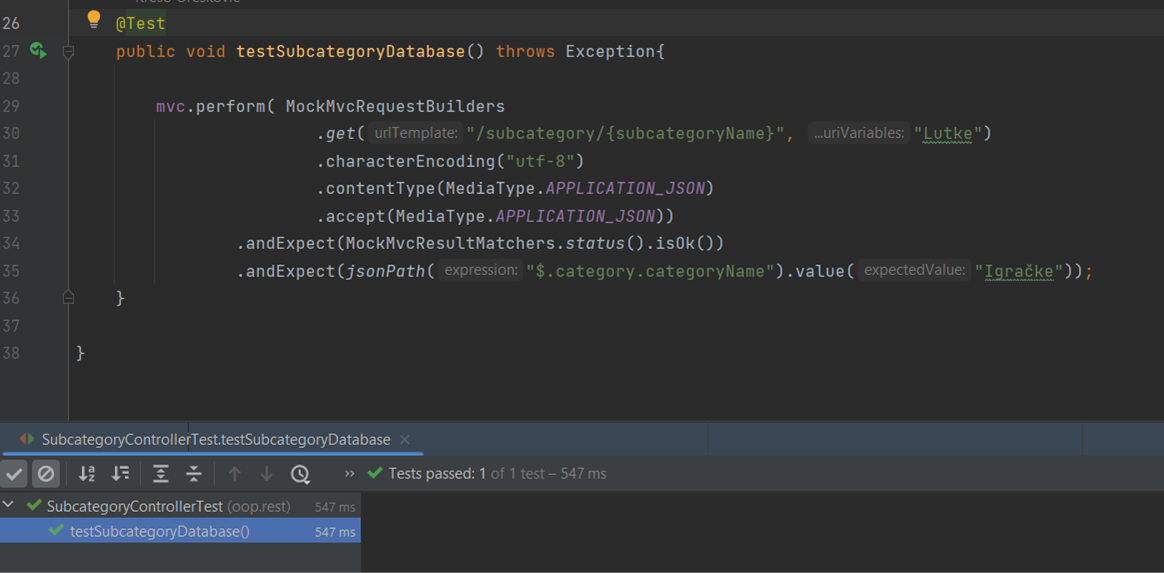
\includegraphics[]{slike/unit1.png}
				\centering
				\caption{Kod prvog unit testa}
				\label{fig:unit1}
			\end{figure}

                \eject

                \subsubsection{Test 2}
                Drugim testom provjerava se dolazi li do pogreške ako pri registraciji korisnik unese mail adresu koja je već unešena u bazi - očekivan je status "400 Bad Request". \underline{Test prolazi.}

                \begin{figure}[H]
				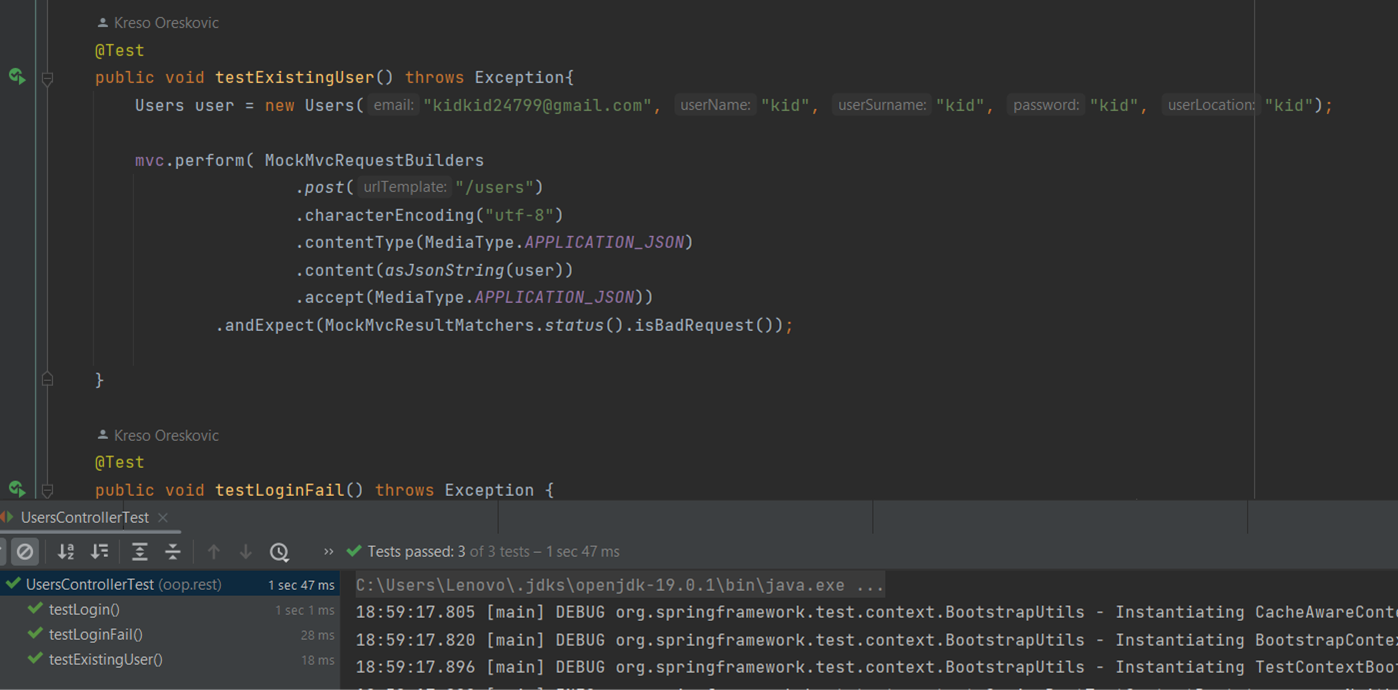
\includegraphics[scale=0.9]{slike/unit2.png}
				\centering
				\caption{Kod drugog unit testa}
				\label{fig:unit2}
			\end{figure}

                \subsubsection{Test 3}
                Trećim testom provjerava se dolazi li do pogreške ako pri loginu korisnik unese mail adresu za koju u bazi ne postoji zapis tj. podaci o korisniku. \underline{Test prolazi.}

                \begin{figure}[H]
				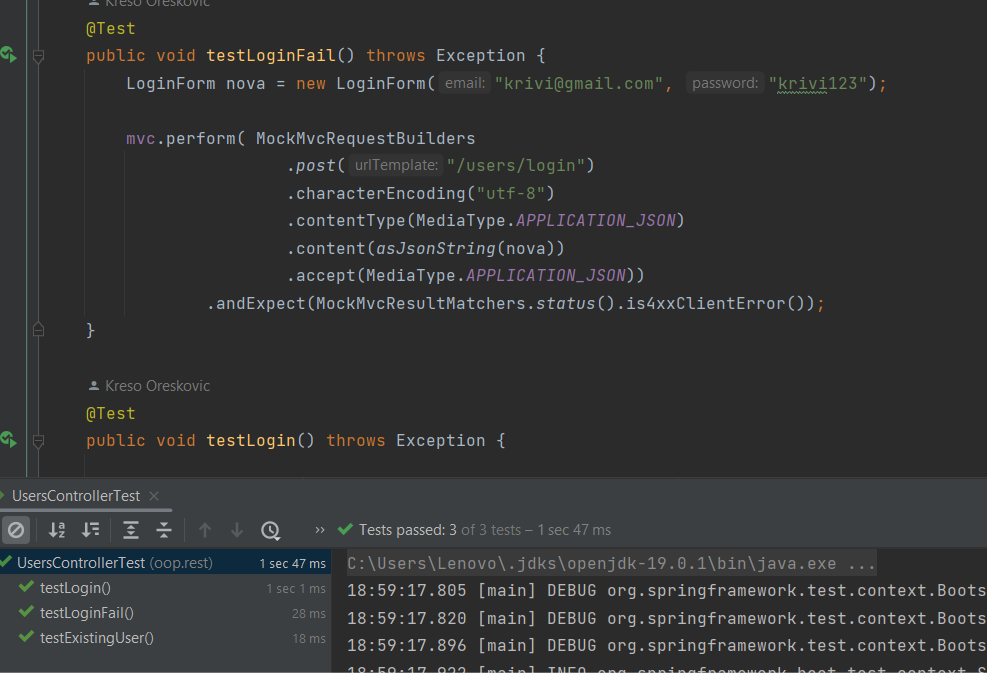
\includegraphics[scale=0.8]{slike/unit3.png}
				\centering
				\caption{Kod trećeg unit testa}
				\label{fig:unit3}
			\end{figure}

                \eject
            
                \subsubsection{Test 4}
                Četvrtim testom provjerava se uspješnost logina korisnika za kojeg u bazi postoje podaci. \underline{Test prolazi.}

                \begin{figure}[H]
				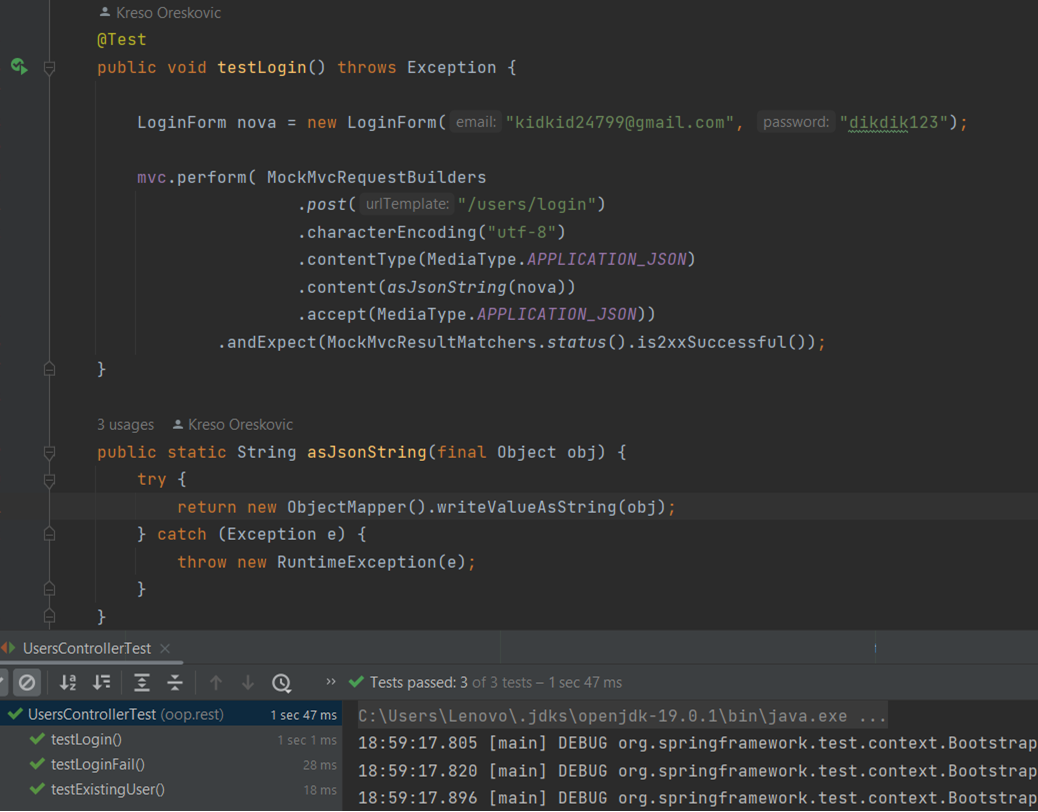
\includegraphics[]{slike/unit4.png}
				\centering
				\caption{Kod četvrtog unit testa}
				\label{fig:unit4}
			\end{figure}

                \subsubsection{Test 5}
                Petim testom provjerava se uspješnost stvaranja donacije. \underline{Test prolazi.}

                \begin{figure}[H]
				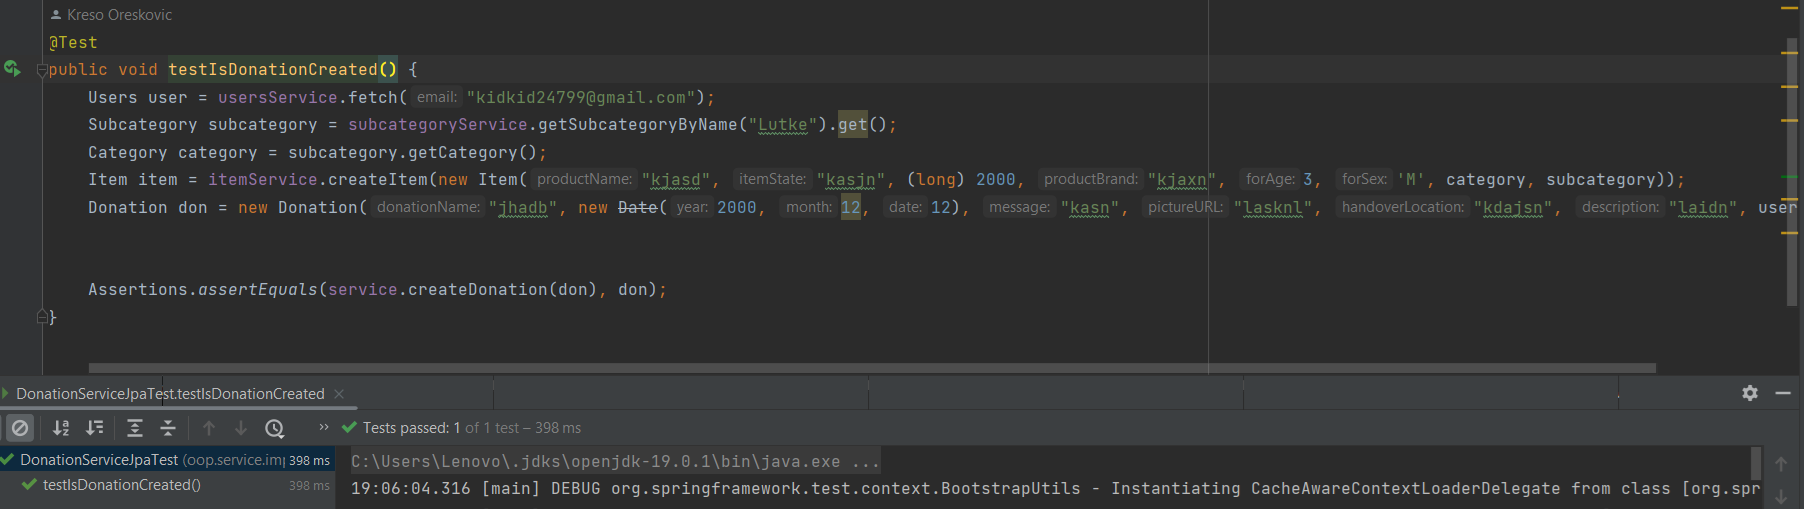
\includegraphics[]{slike/unit5.png}
				\centering
				\caption{Kod petog unit testa}
				\label{fig:unit5}
			\end{figure}

                \subsubsection{Testovi 6, 7}
                Šestim testom provjerava se uspješnost ažuriranja podataka o predmetu. \underline{Test prolazi.}
                Sedmim testom provjerava se uspješnost brisanja predmeta iz baze podataka, kao i dolazi li do "custom" pogreške "EntityMissingException" pri pokušaju dohvaćanja izbrisanog predmeta. \underline{Test prolazi.}

                \begin{figure}[H]
				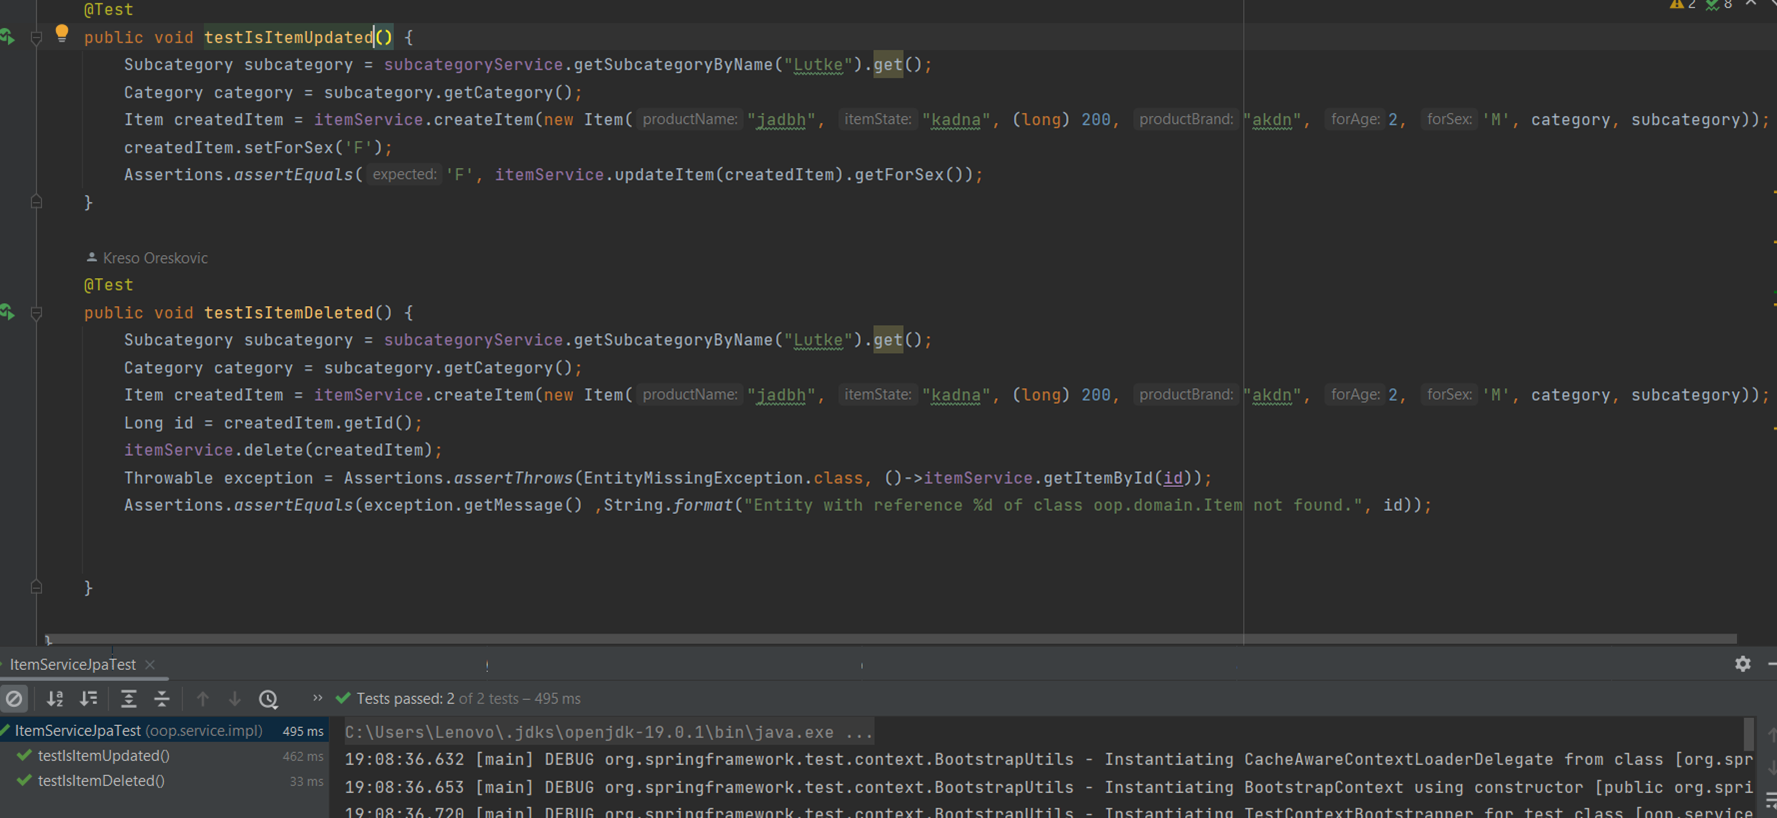
\includegraphics[]{slike/unit6.png}
				\centering
				\caption{Kod šestog i sedmog unit testa}
				\label{fig:unit67}
			\end{figure}

                \subsubsection{Testovi 8, 9}
                Osmim testom provjerava se postoji li admin račun u bazi podataka. \underline{Test prolazi.}
                Devetim testom provjerava se dolazi li do "custom" pogreške "EntityMissingException" pri pokušaju dohvaćanja nepostojećeg korisnika. \underline{Test prolazi.}

                \begin{figure}[H]
				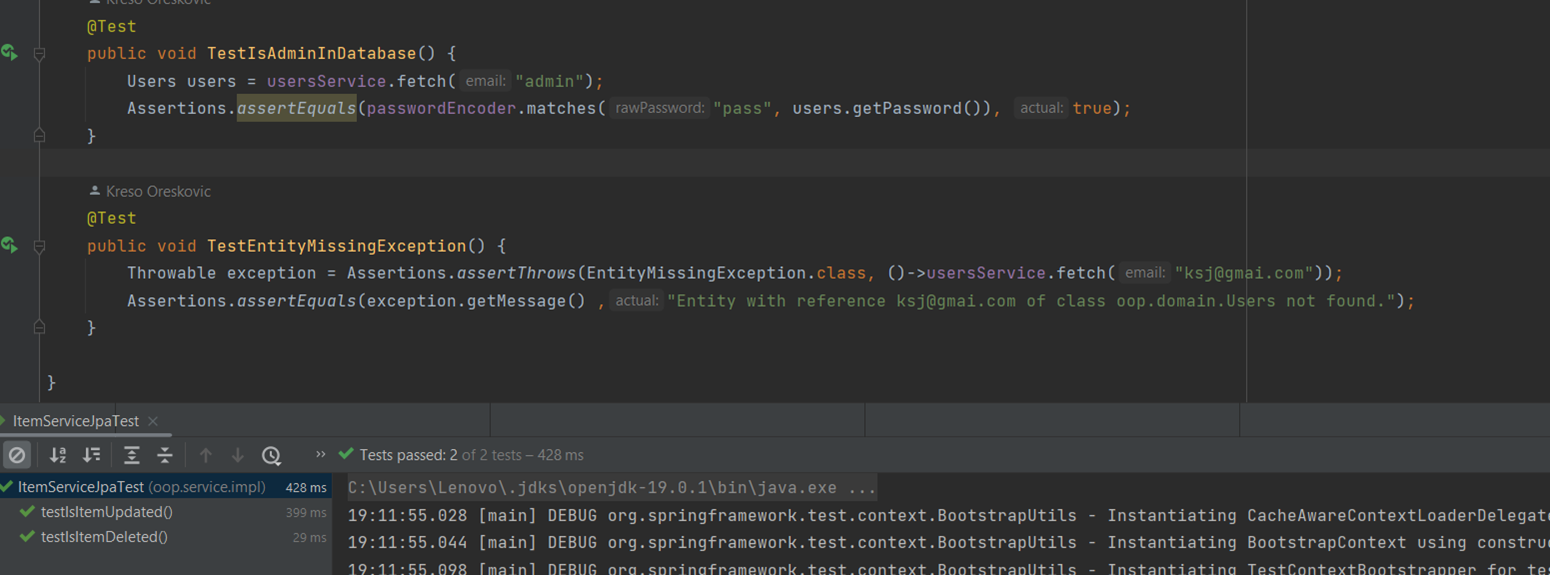
\includegraphics[]{slike/unit7.png}
				\centering
				\caption{Kod osmog i devetog unit testa}
				\label{fig:unit89}
			\end{figure}

                \eject
                
			%\textit{Potrebno je provesti ispitivanje jedinica (engl. unit testing) nad razredima koji implementiraju temeljne funkcionalnosti. 
			%Razraditi \textbf{minimalno 6 ispitnih slučajeva} u kojima će se ispitati redovni slučajevi, rubni uvjeti te izazivanje pogreške (engl. exception throwing). 
			%Poželjno je stvoriti i ispitni slučaj koji koristi funkcionalnosti koje nisu implementirane. 
			%Potrebno je priložiti izvorni kôd svih ispitnih slučajeva te prikaz rezultata izvođenja ispita u razvojnom okruženju (prolaz/pad ispita). }

        
			
			
			
			\subsection{Ispitivanje sustava}

                Za testiranje rada cjelovitog sustava, korišteni su alati Selenium Webdriver i Selenium IDE. Selenium Webdriver omogućava pisanje testova cjelovitog sustava koristeći proizvoljan programski jezik, kao i integraciju tih testova s unit testovima napisanim za testiranje rada pojedinačnih komponenti. S druge strane, Selenium IDE korisnicima omogućava generiranje testova cjelovitog sustava snimanjem svojih akcija i ponavljanjem tih akcija. \\
                
                U našem testiranju, testirali smo funkcionalnosti aplikacije koja je već puštena u pogon (engl. deployana). Pritom smo za jednostavnije funkcionalnosti ručno pisali testove u programskom jeziku Java, dok smo za neke od složenijih funkcionalnosti snimili akcije koristeći alat Selenium IDE. Na slikama vidljiv je kod testova pisanih koristeći Selenium Webdriver, kao i akcije snimljene alatom Selenium IDE. Testovi pisani u programskom jeziku Java izvršeni su zajedno, a rezultat njihovog izvođenja prikazan je na zasebnoj slici. 

                \subsubsection{Test 1}
                Prvim testom provjerava se registracija koristeći već unesenu mail adresu tj. adresu za koju u bazi već postoji zapis o korisniku. Očekivani rezultat izvođenja testa je da ne dolazi do preusmjeravanja na stranicu s prikazom aktivnih oglasa, već je i dalje prikazana stranica za registraciju (s porukom o neuspješnoj registraciji). \underline{Test prolazi.}

                \begin{figure}[H]
				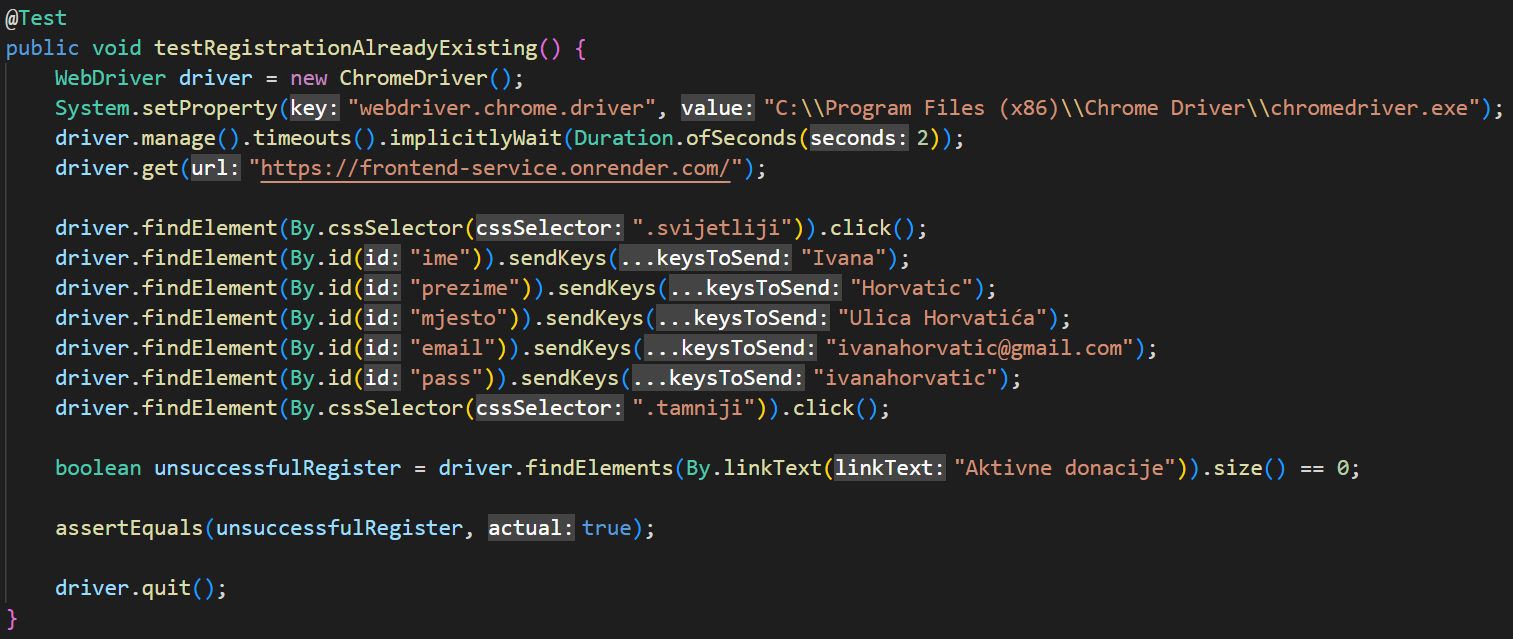
\includegraphics[scale=0.55]{slike/selenium1.png}
				\centering
				\caption{Kod prvog Selenium testa}
				\label{fig:selenium1}
			\end{figure}

                \subsubsection{Test 2}
                Drugim testom provjerava se registracija koristeći ispravne podatke tj. podatke za koje u bazi do sada ne postoji zapis o korisniku. Očekivani rezultat izvođenja testa je da dolazi do preusmjeravanja na stranicu s prikazom aktivnih oglasa koja u zaglavlju ima poveznice na ostale dijelove stranice. \underline{Test prolazi.}

                \begin{figure}[H]
				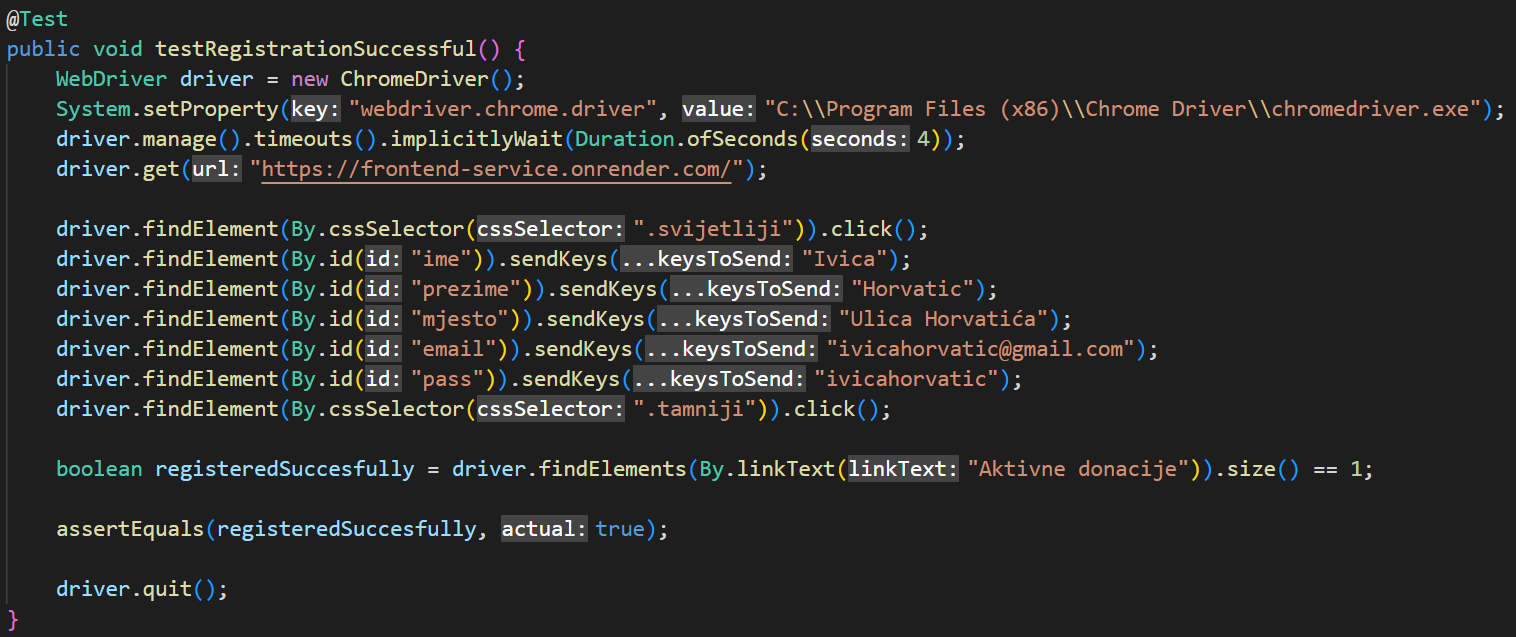
\includegraphics[scale=0.55]{slike/selenium2.png}
				\centering
				\caption{Kod drugog Selenium testa}
				\label{fig:selenium2}
			\end{figure}

                \subsubsection{Test 3}
                Trećim testom provjerava se login korisnika koristeći neispravne podatke (kombinacija ispravna mail adresa, neispravna lozinka korisnika). Očekivani rezultat izvođenja testa je da ne dolazi do preusmjeravanja na stranicu s prikazom aktivnih oglasa, već je i dalje prikazana stranica za login (s porukom o neuspješnoj prijavi). \underline{Test prolazi.}

                \begin{figure}[H]
				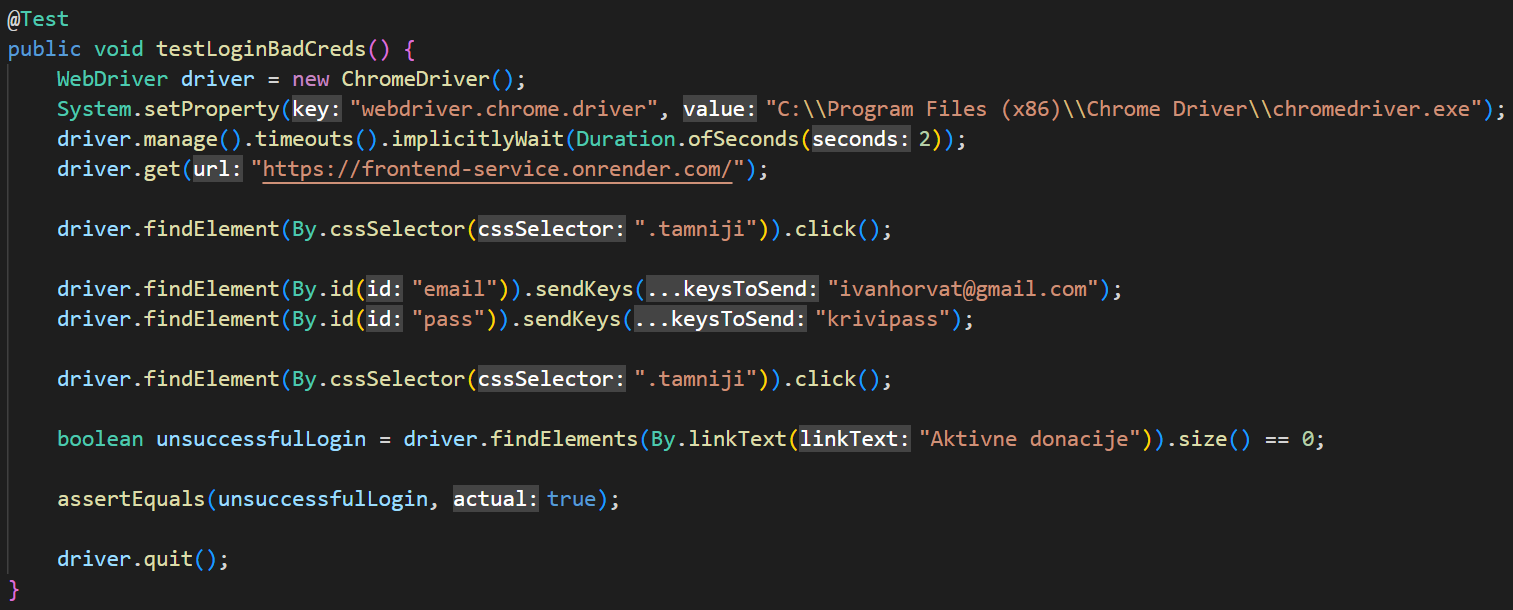
\includegraphics[scale=0.55]{slike/selenium3.png}
				\centering
				\caption{Kod trećeg Selenium testa}
				\label{fig:selenium3}
			\end{figure}

                \subsubsection{Test 4}
                Četvrtim testom provjerava se login korisnika koristeći ispravne podatke (ispravna mail adresa, ispravna lozinka korisnika). Očekivani rezultat izvođenja testa je da dolazi do preusmjeravanja na stranicu s prikazom aktivnih oglasa koja u zaglavlju ima poveznice na ostale dijelove stranice. \underline{Test prolazi.}

                \begin{figure}[H]
				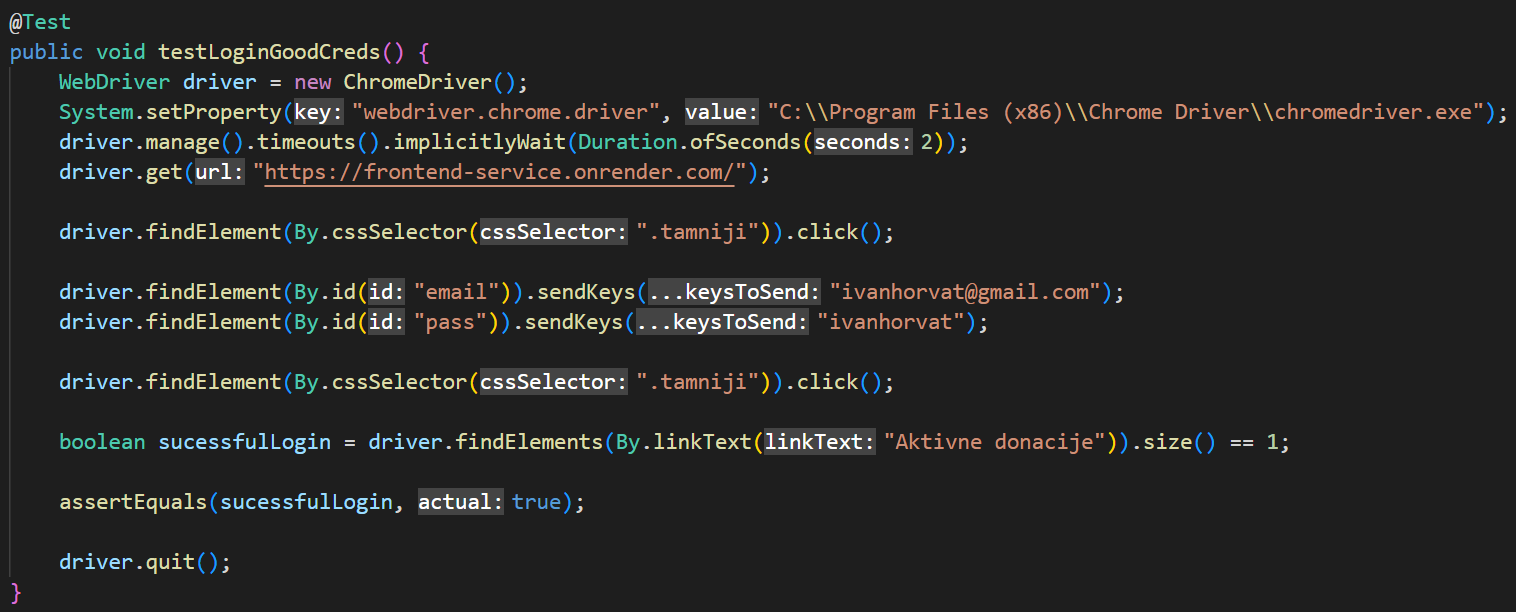
\includegraphics[scale=0.55]{slike/selenium4.png}
				\centering
				\caption{Kod četvrtog Selenium testa}
				\label{fig:selenium4}
			\end{figure}

                \subsubsection{Rezultati izvođenja Selenium testova}
                Na slici 5.12 prikazani su rezultati izvođenja do sada opisanih testova. Sva četiri testa uspješno prolaze, a na slici je prikazano i trajanje pojedinih testova.

                \begin{figure}[H]
				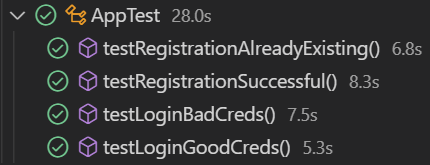
\includegraphics[]{slike/selenium_results.png}
				\centering
				\caption{Rezultati izvođenja Selenium testova}
				\label{fig:seleniumResults}
			\end{figure}

                \eject

                \subsubsection{Test 5}
                Na slici 5.13 prikazane su akcije snimljene koristeći alat Selenium IDE. Alat Selenium IDE korišten je kako bi se preglednije prikazale potrebne akcije - kod za testiranje složenih funkcionalnosti dugačak je i nepregledniji od ovakvog prikaza. Testirano je dodavanje nove kategorije. Kako bi se dodala nova kategorija, korisnik se mora prijaviti koristeći admin podatke. Tijekom provođenja testa, ti su podaci već bili pohranjeni u pregledniku pa je bilo dovoljno kliknuti na gumb za prijavu. Nakon uspješne prijave, dolazimo do stranice za dodavanje kategorija i potkategorija te pokušavamo stvoriti novu kategoriju proizvoljnog imena. \underline{Test prolazi.}

                \begin{figure}[H]
                \makebox[\textwidth][c]{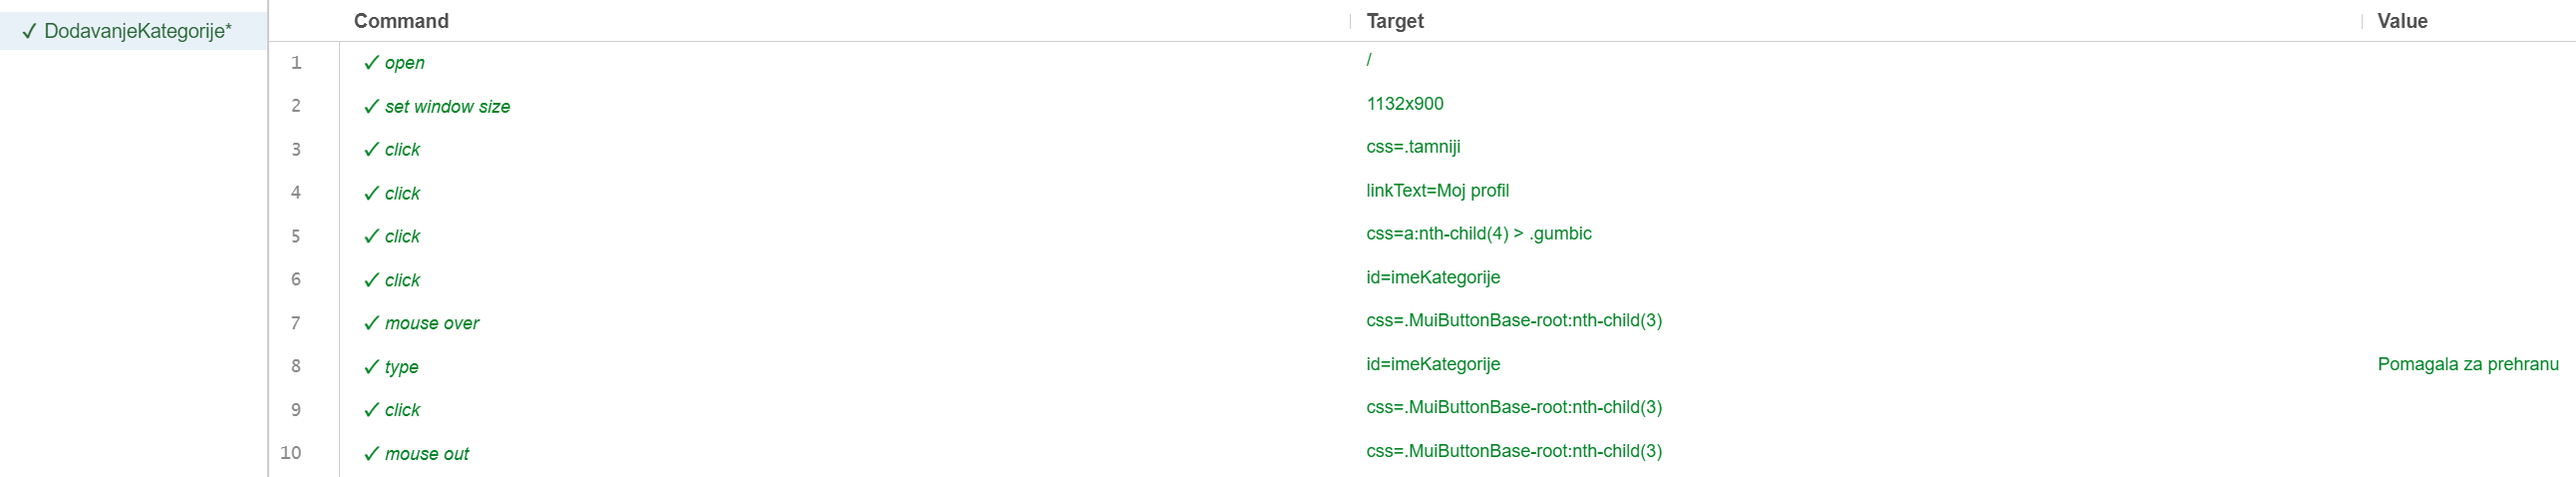
\includegraphics[scale=0.4]{slike/selenium5.png}}%
				\centering
				\caption{Akcije petog Selenium testa}
				\label{fig:selenium5}
			\end{figure}

                Uz pet do sada prikazanih Selenium testova, dodatno su testirane i funkcionalnosti stvaranja oglasa, dodavanja potkategorije i uređivanja podataka, ali zbog preglednosti i sažetosti ti testovi nisu uključeni u dokumentaciju. 

                \eject
			
			 %\textit{Potrebno je provesti i opisati ispitivanje sustava koristeći radni okvir Selenium\footnote{\url{https://www.seleniumhq.org/}}. 
			 %Razraditi \textbf{minimalno 4 ispitna slučaja} u kojima će se ispitati redovni slučajevi, 
			% rubni uvjeti te poziv funkcionalnosti koja nije implementirana/izaziva pogrešku kako bi se vidjelo na koji način sustav reagira kada nešto nije u potpunosti ostvareno. 
			 %Ispitni slučaj se treba sastojati od ulaza (npr. korisničko ime i lozinka), očekivanog izlaza ili rezultata, koraka ispitivanja i dobivenog izlaza ili rezultata.\\ }
			 
			 %\textit{Izradu ispitnih slučajeva pomoću radnog okvira Selenium moguće je provesti pomoću jednog od sljedeća dva alata:}
			 %\begin{itemize}
			 	%\item \textit{dodatak za preglednik \textbf{Selenium IDE} - snimanje korisnikovih akcija radi automatskog ponavljanja ispita	}
			 	%\item \textit{\textbf{Selenium WebDriver} - podrška za pisanje ispita u jezicima Java, C\#, PHP koristeći posebno programsko sučelje.}
			 %\end{itemize}
		 	%\textit{Detalji o korištenju alata Selenium bit će prikazani na posebnom predavanju tijekom semestra.}
			
			%\eject 
		
		
		\section{Dijagram razmještaja}
			
			%\textbf{\textit{dio 2. revizije}}

                Dijagram razmještaja opisuje konkretno ostvarenje odabrane arhitekture aplikacije - na slici 5.14 moguće je vidjeti raspodjelu programske potpore na konkretno sklopovlje. Kod za prikaz korisničkog sučelja i komunikaciju s korisnikom pisan u React.js pušten je u pogon na platformi Render. Kako bi aplikacija bila funkcionalna, u pogon su zasebno pušteni (engl. deployani) baza podataka ostvarena koristeći PostgreSQL te kod za poslovnu logiku i komunikaciju s bazom (backend) pisan u Java Spring Boot-u. Kako bi kod za backend bio uspješno deployan, za njega postoji i Docker container koji osigurava da je u njemu ispravno "spakiran" sav kod, kao i zavisnosti potrebne za uspješan rad istoga. I backend i baza podataka pušteni su u pogon koristeći platformu Render. \\

                Uz ovo, na platformi Firebase napravljen je Cloud Storage Bucket koji služi za jednostavnu pohranu slika potrebnih za uspješan prikaz oglasa. Komunikacija između zasebnih uređaja i platformi osigurana je protokolom HTTPS (komunikacija između klijentovog računala tj. web preglednika na istome i web poslužitelja deployanog na platformi Render, kao i komunikacija između web poslužitelja i Cloud Storage Bucket-a deployanog na platformi Firebase). Kako bi web poslužitelj korisniku mogao poslužiti sav potreban sadržaj, on komunicira s backendom koji po potrebi komunicira s bazom podataka.

                \begin{figure}[H]
				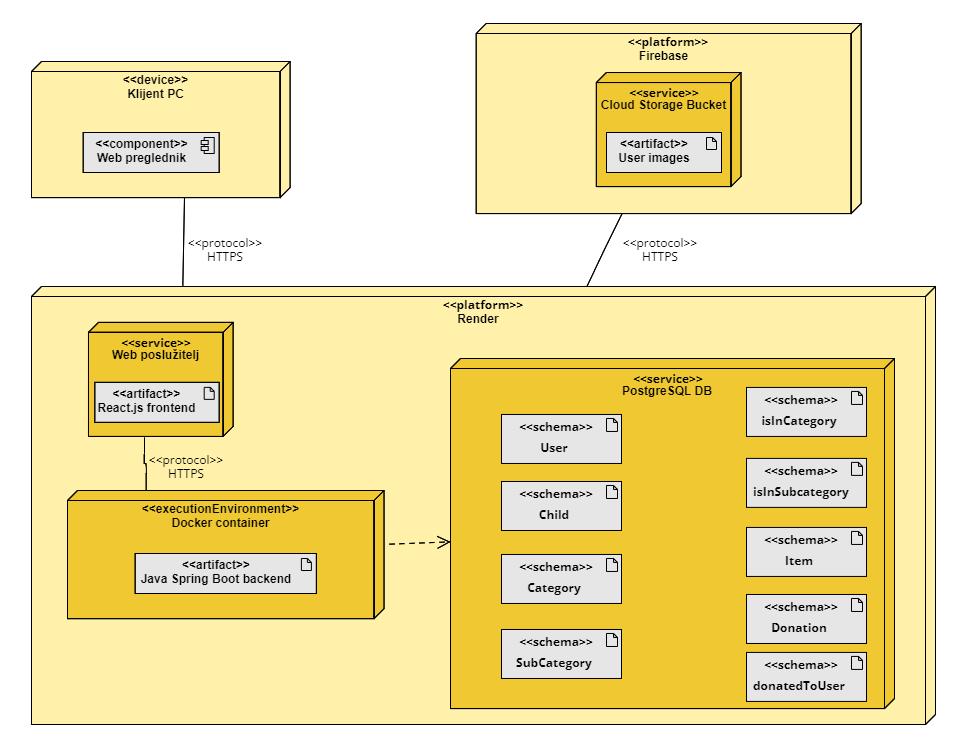
\includegraphics[width=\textwidth,height=0.8\textheight]{dijagrami/Dijagram razmjestajav2.png}
				\centering
				\caption{Dijagram razmještaja}
				\label{fig:DeploymentDiagram}
			\end{figure}
			
			\eject 
		
		\section{Upute za puštanje u pogon}
		
			%\textbf{\textit{dio 2. revizije}}\\
                Frontend, backend i baza podatka puštene su u pogon na platformi Render. Upute za pristupanje platformi Render, kao i upute za puštanje u pogon (engl. deploy) slijede u sljedećim sekcijama.
          
			    \subsection{Pristupanje Renderu}

                Kako bi pristupili Renderu, prilikom prijave u web aplikaciju koristimo GitLab račune koji se direktno mogu povezati s njime. Povezivanjem Gitlab računa s platformom Render dobivamo lakši pristup kodu koji će se pustiti u pogon.

                \begin{figure}[H]
				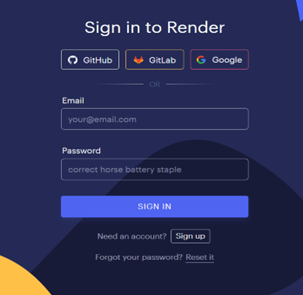
\includegraphics[width=0.6\textwidth,height=0.3\textheight]{slike/renderSignIn.png}
				\centering
				\caption{Render sign in}
				\label{fig:renderSignIn}
			\end{figure}

                \subsection{Backend deploy na Render}

                \textbf{1. Priprema}\\
                
                Prije puštanja aplikacije u pogon na Renderu potrebno je u izvorni kod za backend dodati Dockerfile za Maven projekt te u datoteci application.properties postaviti property server.servlet.context-path na /api da bude prefiks svim zahtjevima na backend.
			
			\eject 

                \textbf{2. Kreiranje baze podataka}\\

                U render dashboard potrebno je:

                \begin{itemize}
                    \item Pritisnuti tipku New te onda odabrati opciju PostgreSQL za kreiranje baze
                    \begin{figure}[H]
    			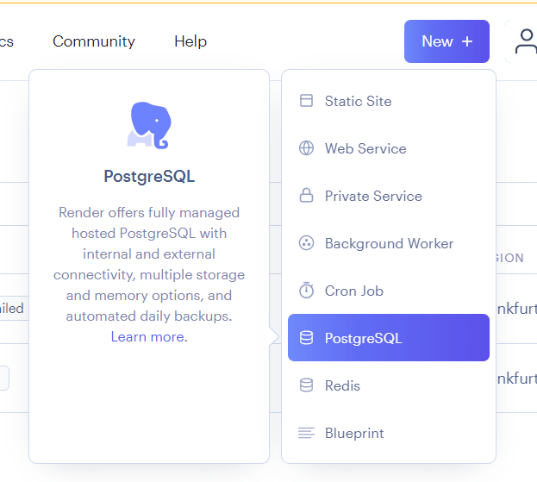
\includegraphics[width=0.6\textwidth,height=0.3\textheight]{slike/postgresqlCreate.png}
    			\centering
    			\caption{Kreiranje nove PostgreSQL baze}
    			\label{fig:newPostgreSQLDB}
    			\end{figure}
                    \item Postaviti ime baze
                    \item Database i User ostaviti prazno jer se automatski generira pri kreiranju baze
                    \item Postaviti Region na Frankfurt
                    \item Pritisnuti Create Database
                \end{itemize}

                \begin{figure}[H]
				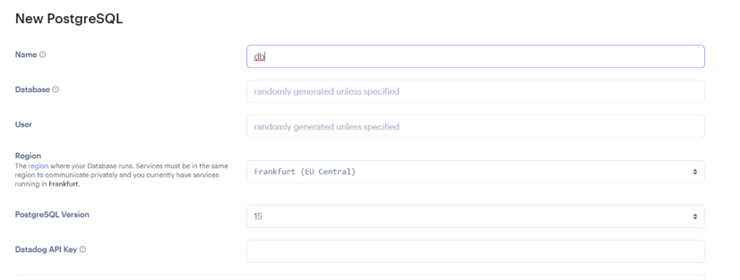
\includegraphics[width=0.8\textwidth,height=0.25\textheight]{slike/postgresqlNew.png}
				\centering
				\caption{Ispunjavanje podataka o bazi}
				\label{fig:postgresqlFillData}
			\end{figure}

                Prije puštanja backend-a u pogon, u datoteci application.properties moramo uvrstiti username, password za pristup bazi, database, hostname i port za url prema bazi na koju se treba spojiti.

                \begin{figure}[H]
				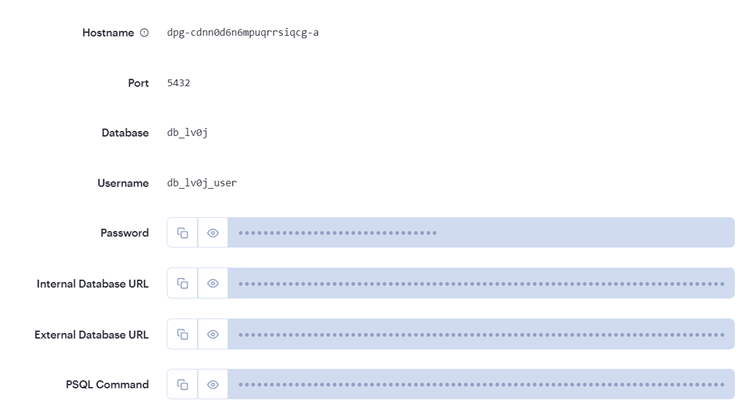
\includegraphics[width=0.8\textwidth,height=0.25\textheight]{slike/postgresqlNewFilled.png}
				\centering
				\caption{Ispunjavanje podataka u datoteci application.properties}
				\label{fig:applicationPropertiesDB}
			\end{figure}

                \textbf{3. Kreiranje backenda}\\

                U Render dashboard potrebno je:

                \begin{itemize}
                    \item Pritisnuti tipku New te onda odabrati opciju Web Service za kreiranje web usluge
                    \item Povezati GitLab račun - nakon povezivanja su za odabir dostupni svi projekti na koje imate prava pristupa
                    \item Pritisnuti Connect pokraj odgovarajućeg projekta
                    \begin{figure}[H]
    			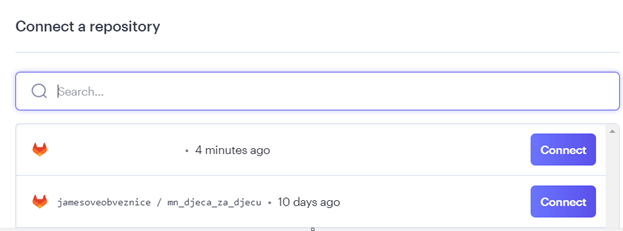
\includegraphics[width=0.8\textwidth,height=0.25\textheight]{slike/connectRepo.png}
    			\centering
    			\caption{Povezivanje repozitorija}
    			\label{fig:connectRepo}
    			\end{figure}
                    \item Postaviti ime za servis (ime servisa na kraju će biti dio web adrese)
                    \item Root directory postaviti na IzvorniKod/backend
                    \item Environment postaviti na Docker
                    \item Region postaviti na Frankfurt
                    \begin{figure}[H]
    			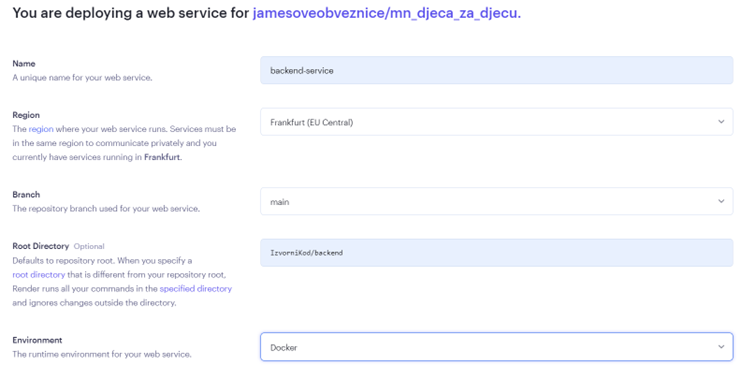
\includegraphics[width=0.8\textwidth,height=0.25\textheight]{slike/deployWebService.png}
    			\centering
    			\caption{Podaci za puštanje web servisa u pogon}
    			\label{fig:deployWebService}
    			\end{figure}
                    \item Na dnu proširiti \textit{advanced}
                    \item Postaviti putanju za Dockerfile ovisno koji se package manager koristi (u ovom slučaju putanja je ./docker/maven/Dockerfile)
                    \begin{figure}[H]
                    \makebox[\textwidth][c]{
\includegraphics[]{slike/dockerfilePath.png}}%
    			\centering
    			\caption{Putanja Dockerfile-a}
    			\label{fig:dockerFilePath}
    			\end{figure}
                    \item Pritisnuti Create Web Service
                \end{itemize}

                Nakon izvođenja svih ovih koraka, u pogon bi se trebala uspješno pustiti (eng. deployati) backend aplikacija. Nakon puštanja backend aplikacije u pogon, isto ćemo napraviti i za frontend aplikaciju.

                \eject

                \subsection{Frontend deploy na Render}

                Kako bi se frontend uspješno pustio u pogon, u Render dashboard potrebno je:

                \begin{itemize}
                    \item Pritisnuti tipku New i odabrati opciju Web Service za kreiranje web usluge
                    \item Povezati GitLab račun - nakon povezivanja su za odabir dostupni svi projekti na koje imate prava pristupa
                    \item Pritisnuti Connect pokraj odgovarajućeg projekta
                    \begin{figure}[H]
    			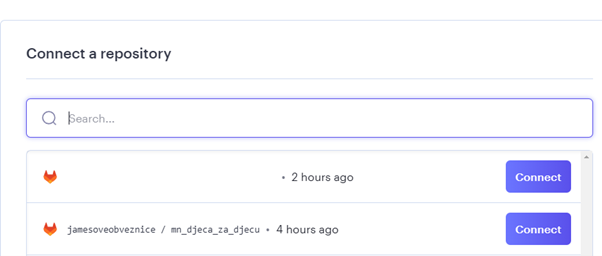
\includegraphics[width=\textwidth,height=0.25\textheight]{slike/connectFront.png}
    			\centering
    			\caption{Povezivanje repozitorija za frontend}
    			\label{fig:connectRepoFront}
    			\end{figure}
                    \item Postaviti ime za servis (ime servisa na kraju će biti dio web adrese)
                    \item Root directory postaviti na IzvorniKod/Frontend/dzd-app/
                    \item Environment postaviti na Node
                    \begin{figure}[H]
    			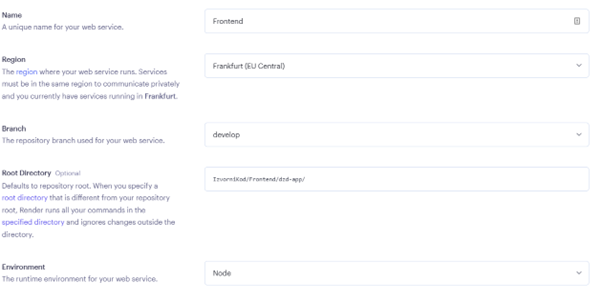
\includegraphics[scale=0.75]{slike/fillDataDeployFront.png}
    			\centering
    			\caption{Ispunjavanje podataka o frontendu}
    			\label{fig:fillDataFront}
    			\end{figure}
                    \item Region postaviti na Frankfurt
                    \item Odabrati branch iz kojeg se uzimaju datoteke za frontend
                    \item Build Command postaviti na yarn build
                    \item Start Command postaviti na yarn start-prod
                    \begin{figure}[H]
    			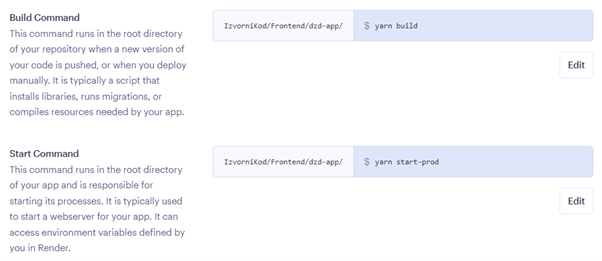
\includegraphics[]{slike/buildFront.png}
    			\centering
    			\caption{Unošenje ispravnih naredbi}
    			\label{fig:buildFrontCommands}
    			\end{figure}\textbf{}
                    \item Na dnu pritisnuti Advanced
                    \item Dodati potrebne Environment varijable - API\_BASE\_URL postaviti na adresu deployanog backenda aplikacije dostupnu na Render dashboardu
                    \item Isključiti Auto-Deploy kako se projekt ne bi ponovno deployao za svaki novi commit
                    \item Pritisnuti Create Web Service
                \end{itemize}

                Nakon izvođenja svih ovih koraka, u pogon bi se trebala uspješno pustiti (eng. deployati) frontend aplikacija. Stranici pristupamo preko URL-a za \underline{frontend}\footnote{\url{https://frontend-service.onrender.com/}}.
	\chapter{Zaključak i budući rad}
		
		\textbf{\textit{dio 2. revizije}}\\
		
		 \textit{U ovom poglavlju potrebno je napisati osvrt na vrijeme izrade projektnog zadatka, koji su tehnički izazovi prepoznati, jesu li riješeni ili kako bi mogli biti riješeni, koja su znanja stečena pri izradi projekta, koja bi znanja bila posebno potrebna za brže i kvalitetnije ostvarenje projekta i koje bi bile perspektive za nastavak rada u projektnoj grupi.}
		
		 \textit{Potrebno je točno popisati funkcionalnosti koje nisu implementirane u ostvarenoj aplikaciji.}
		
		\eject 
	\chapter*{Popis literature}
		\addcontentsline{toc}{chapter}{Popis literature}
	 	
 		%\textbf{\textit{Kontinuirano osvježavanje}}
	
		%\textit{Popisati sve reference i literaturu koja je pomogla pri ostvarivanju projekta.}
		
		
		\begin{enumerate}
			
			
			\item  Programsko inženjerstvo, FER ZEMRIS, \url{http://www.fer.hr/predmet/proinz}
			
			\item  I. Sommerville, "Software engineering", 8th ed, Addison Wesley, 2007.
			
			\item  T.C.Lethbridge, R.Langaniere, "Object-Oriented Software Engineering", 2nd ed. McGraw-Hill, 2005.
			
			\item  I. Marsic, Software engineering book``, Department of Electrical and Computer Engineering, Rutgers University, \url{http://www.ece.rutgers.edu/~marsic/books/SE}
			
			\item  The Unified Modeling Language, \url{https://www.uml-diagrams.org/}
			
			\item  Visual Paradigm, \url{https://www.visual-paradigm.com/}
		\end{enumerate}
		
		 
	
	
	\begingroup
	\renewcommand*\listfigurename{Indeks slika i dijagrama}
	%\renewcommand*\listtablename{Indeks tablica}
	%\let\clearpage\relax
	\listoffigures
	%\vspace{10mm}
	%\listoftables
	\endgroup
	\addcontentsline{toc}{chapter}{Indeks slika i dijagrama}


	
	\eject 
		
	\chapter*{Dodatak: Prikaz aktivnosti grupe}
		\addcontentsline{toc}{chapter}{Dodatak: Prikaz aktivnosti grupe}
		
		\section*{Dnevnik sastajanja}
		
		%\textbf{\textit{Kontinuirano osvježavanje}}\\
		
		% \textit{U ovom dijelu potrebno je redovito osvježavati dnevnik sastajanja prema predlošku.}
		
		\begin{packed_enum}
			\item  sastanak
			
			\item[] \begin{packed_item}
				\item Datum: 14. listopada 2022
				\item Prisustvovali: D.Kiramarios, D.Kovačević, K.Tomičić, D.Jambrović, K.Orešković, K.Kijac, S.Barac
				\item Teme sastanka:
				\begin{packed_item}
					\item  raspodjela uloga (podjela poslova na frontend, backend i razvoj dokumentacije)
					\item  rasprava o zadanoj temi
					\item  sakupljanje pitanja za prvi sastanak sa asistenticom
				\end{packed_item}
			\end{packed_item}
			
			\item  sastanak
			\item[] \begin{packed_item}
				\item Datum: 20. listopada 2022
				\item Prisustvovali: D.Kiramarios, D.Kovačević, K.Tomičić, D.Jambrović, K.Orešković, K.Kijac, S.Barac
				\item Teme sastanka:
				\begin{packed_item}
					\item  osnovni podaci o izvođenju projekta
					\item  postavljanje pitanja vezanih za implementaciju projekta asistentici tijekom prvih pola sata sastanka i sljedećih 20 min
				\end{packed_item}
			\end{packed_item}

			\item  sastanak
			\item[] \begin{packed_item}
				\item Datum: 20. listopada 2022
				\item Prisustvovali: D.Kiramarios, D.Kovačević, K.Tomičić, D.Jambrović, K.Orešković, K.Kijac, S.Barac
				\item Teme sastanka:
				\begin{packed_item}
					\item  detaljna analiza zadatka
					\item  planiranje raspodjele poslova tijekom sljedećeg tjedna vezanih za inicijalizaciju backenda, frontenda i dokumentacije
					\item  dogovor o korištenju Jire za bolje praćenje raspodjele poslova
				\end{packed_item}
			\end{packed_item}

			\eject

			\item  sastanak
			\item[] \begin{packed_item}
				\item Datum: 23. listopada 2022
				\item Prisustvovali: D.Kiramarios, D.Kovačević, K.Tomičić, D.Jambrović, K.Orešković, K.Kijac, S.Barac
				\item Teme sastanka:
				\begin{packed_item}
					\item  pregled predložene skice klijentske aplikacije (frontend)
					\item  pregled predložene sheme za bazu podataka (backend)
					\item  pregled obrazaca uporabe i UC dijagrama (dokumentacija)
					\item  zaključak: male promjene sheme baze i slanje na pregled asistentici
				\end{packed_item}
			\end{packed_item}

			\item  sastanak
			\item[] \begin{packed_item}
				\item Datum: 24. listopada 2022
				\item Prisustvovali: D.Kiramarios, K.Tomičić, S.Barac
				\item Teme sastanka:
				\begin{packed_item}
					\item  detaljna analiza prijedloga dizajna za klijentsku aplikaciju
					\item  male promjene dizajna za klijentsku aplikaciju
					\item  podjela posla na klijentskoj aplikaciji među prisutnima
				\end{packed_item}
			\end{packed_item}

			\item  sastanak
			\item[] \begin{packed_item}
				\item Datum: 31. listopada 2022
				\item Prisustvovali: D.Kiramarios, K.Tomičić, S.Barac
				\item Teme sastanka:
				\begin{packed_item}
					\item  podjela posla na izradu routinga, izgleda, određenih komponenti i spajanja s backendom
				\end{packed_item}
			\end{packed_item}

			\item  sastanak
			\item[] \begin{packed_item}
				\item Datum: 3. studenoga 2022
				\item Prisustvovali: D.Kiramarios, D.Kovačević, K.Tomičić, D.Jambrović, K.Orešković, K.Kijac, S.Barac
				\item Teme sastanka:
				\begin{packed_item}
					\item pregled napravljene dokumentacije s asistenticom
					\item savjeti oko potrebnih promjena dokumentacije
					\item razgovor o implementaciji konkretnih svari na frontendu i backendu
				\end{packed_item}
			\end{packed_item}

			\eject

			\item  sastanak
			\item[] \begin{packed_item}
				\item Datum: 5. studenoga 2022
				\item Prisustvovali: K.Kijac, D.Jambrović
				\item Teme sastanka:
				\begin{packed_item}
					\item pregled prve verzije dokumentacije
					\item podjela posla oko finalnih promjena prve verzije dokumentacije
				\end{packed_item}
			\end{packed_item}

			\item  sastanak
			\item[] \begin{packed_item}
				\item Datum: 8. studenoga 2022
				\item Prisustvovali: D.Kiramarios, D.Kovačević, K.Orešković, S.Barac
				\item Teme sastanka:
				\begin{packed_item}
					\item spajanje frontenda i backenda (integracija API poziva)
				\end{packed_item}
			\end{packed_item}

			\item  sastanak
			\item[] \begin{packed_item}
				\item Datum: 9. studenoga 2022
				\item Prisustvovali: D.Kiramarios, K.Tomičić, S.Barac
				\item Teme sastanka:
				\begin{packed_item}
					\item daljnji planovi oko podjele posla na frontendu
					\item priprema za deploy prve inačice
				\end{packed_item}
			\end{packed_item}

			\item  sastanak
			\item[] \begin{packed_item}
				\item Datum: 10. studenoga 2022
				\item Prisustvovali: K.Orešković, D.Jambrović
				\item Teme sastanka:
				\begin{packed_item}
					\item pregled i diskusija dijagrama razreda
				\end{packed_item}
			\end{packed_item}
			
		\end{packed_enum}
		
		\eject
		\section*{Tablica aktivnosti}
		
			%\textbf{\textit{Kontinuirano osvježavanje}}\\
			
			 \textit{Napomena: Doprinose u aktivnostima treba navesti u satima po članovima grupe po aktivnosti.}

			\begin{longtblr}[
					label=none,
				]{
					vlines,hlines,
					width = \textwidth,
					colspec={X[7, l]X[1, c]X[1, c]X[1, c]X[1, c]X[1, c]X[1, c]X[1, c]}, 
					vline{1} = {1}{text=\clap{}},
					hline{1} = {1}{text=\clap{}},
					rowhead = 1,
				} 
				\multicolumn{1}{c|}{}
				& \multicolumn{1}{c|}{\rotatebox{90}{\textbf{Dario Kiramarios }}}
				& \multicolumn{1}{c|}{\rotatebox{90}{\textbf{David Kovačević }}}
				& \multicolumn{1}{c|}{\rotatebox{90}{\textbf{Krunoslav Tomičić }}}
				& \multicolumn{1}{c|}{\rotatebox{90}{\textbf{Dominik Jambrović }}}
				& \multicolumn{1}{c|}{\rotatebox{90}{\textbf{Krešo Orešković }}} 
				& \multicolumn{1}{c|}{\rotatebox{90}{\textbf{Karla Kijac }}}
				& \multicolumn{1}{c|}{\rotatebox{90}{\textbf{Sven Barac }}} \\  
				Upravljanje projektom 		& 6 & 5 & 5 & 5 & 5 & 5 & 5\\ 
				Opis projektnog zadatka 	&  &  &  & 2 &  & 7 & \\ 
				Funkcionalni zahtjevi       &  &  &  & 2 &  &  &  \\ 
				Opis pojedinih obrazaca 	&  &  &  & 6 &  &  &  \\ 
				Dijagram obrazaca 			&  &  &  & 5 &  & 5 &  \\ 
				Sekvencijski dijagrami 		&  &  &  &  &  &  &  \\ 
				Opis ostalih zahtjeva 		&  &  &  & 1 &  &  &  \\ 
				Arhitektura i dizajn sustava	 &  &  &  & 1 &  &  &  \\ 
				Baza podataka				&  &  &  & 4 &  &  &   \\ 
				Dijagram razreda 			&  &  &  &  & 3 &  &   \\ 
				Dijagram stanja				&  &  &  &  &  &  &  \\ 
				Dijagram aktivnosti 		&  &  &  &  &  &  &  \\ 
				Dijagram komponenti			&  &  &  &  &  &  &  \\ 
				Korištene tehnologije i alati 		&  &  &  &  &  &  &  \\ 
				Ispitivanje programskog rješenja 	&  &  &  &  &  &  &  \\ 
				Dijagram razmještaja			&  &  &  &  &  &  &  \\ 
				Upute za puštanje u pogon 		&  &  &  &  &  &  &  \\  
				Dnevnik sastajanja 			&  &  &  & 3 &  &  &  \\ 
				Zaključak i budući rad 		&  &  &  &  &  &  &  \\  
				Popis literature 			&  &  &  &  &  & 1 &  \\  
				\hline
				\textit{Front end} 				& 10 &  & 10 &  &  &  & 10 \\  
				\textit{Izrada baze podataka} 		 			&  & 5 &  &  & 5 &  & \\  
				\textit{Spajanje s bazom podataka} 				& 2 & 2 & 2 &  & 2 &  & 2 \\ 
				\textit{Back end} 							&  & 10 &  &  & 10 &  &  \\  
				\textit{Popravak dokumentacije}			&  &  &  & 3 &  &  &  \\  
			\end{longtblr}
					
					
		\eject
		\section*{Dijagrami pregleda promjena}
		
		%\textbf{\textit{dio 2. revizije}}\\
		
		%unos slike
		\begin{figure}[H]
			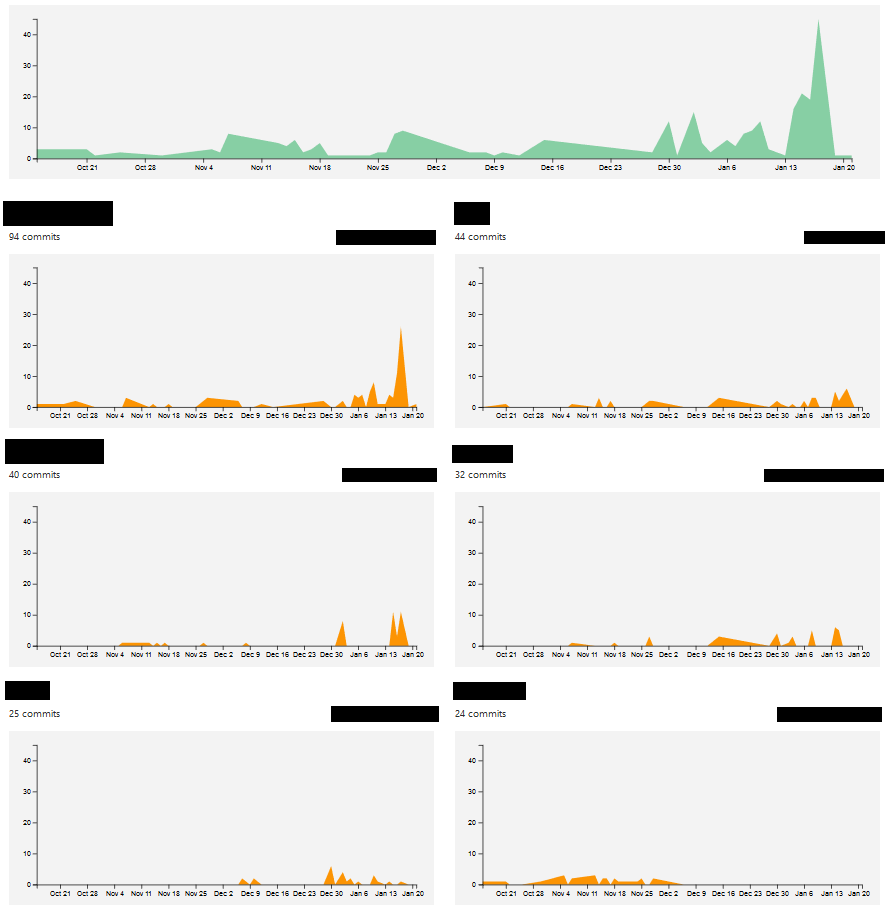
\includegraphics[scale=0.4]{slike/aktivnost.PNG}
			\centering
			\caption{Primjer slike s potpisom}
			\label{fig:promjene}
		\end{figure}


\end{document} %naredbe i tekst nakon ove naredbe ne ulaze u izgrađen dokument 


